\documentclass[12pt, a4paper]{report}

% === PACKAGE IMPORTS ===
\usepackage[utf8]{inputenc}
\usepackage[T1]{fontenc}
\usepackage{graphicx}
\usepackage{amsmath}
\usepackage{setspace}
\usepackage[margin=1in]{geometry}
\usepackage{fancyhdr}
\usepackage{xcolor}
\usepackage{hyperref}
\usepackage{booktabs}
\usepackage{caption}
\usepackage{cite}
\usepackage{svg}
\usepackage{float}
\usepackage{multirow}
\usepackage{array}
\usepackage{longtable}

\setlength{\headheight}{14.49998pt}
\onehalfspacing

\pagestyle{fancy}
\fancyhf{}
\fancyhead[L]{\nouppercase{\leftmark}}
\fancyhead[R]{\thepage}
\renewcommand{\headrulewidth}{0.4pt}
\renewcommand{\chaptermark}[1]{\markboth{\thechapter.\ #1}{}}

\newcommand{\keyresult}[1]{\textcolor{blue!60!black}{\textbf{#1}}}

\hypersetup{
    colorlinks=true,
    linkcolor=blue!50!black,
    citecolor=green!60!black,
    urlcolor=magenta!70!black,
    pdftitle={Multi-Layered Malware Detection and Threat Prevention System},
    pdfauthor={Sangam Kumar Mishra}
}

\begin{document}

% --- TITLE PAGE ---
\begin{titlepage}
    \centering
    \vspace*{0.5cm}
    \includesvg[width=0.22\textwidth]{logo}
    \vspace{0.8cm}

    {\large \textsc{Indian Institute of Technology Bhubaneswar}}\\[0.25cm]
    {\large \textsc{School of Electrical and Computer Sciences}}\\[1.2cm]

    \hrulefill\\[0.4cm]
    {\bfseries\LARGE Multi-Layered Malware Detection and Threat Prevention System}\\[0.4cm]
    \hrulefill\\[1.2cm]

    {\small A B.Tech Project Report Submitted in Partial Fulfillment of the Requirements for the Degree of}\\[0.3cm]
    {\large \textbf{Bachelor of Technology}}\\[1.0cm]

    {\small by}\\[0.2cm]
    {\large \textbf{Sangam Kumar Mishra}}\\[0.1cm]
    {\small (Roll No: 22cs01071)}\\[1.2cm]

    {\small Under the Guidance of}\\[0.2cm]
    {\large \textbf{Prof. Padmalochan Bera}}\\[0.1cm]
    {\small Department of Computer Science and Engineering}\\[0.5cm]

    {\large May 2026}\\[0.2cm]

    \vspace*{\fill}
\end{titlepage}

% --- ABSTRACT ---
\chapter*{Abstract}
\addcontentsline{toc}{chapter}{Abstract}
\thispagestyle{plain}

Modern cyber-physical systems such as drone fleets continuously capture large
volumes of video, imagery, telemetry, and mission metadata. These streams must
be inspected in real time for malware, tampering, covert exfiltration attempts,
and payload manipulation. Traditional single-layer malware scanners struggle
against encrypted archives, polymorphic malware, and payloads hidden inside
multi-modal drone data.

This project designs and implements a \textbf{multi-layered threat prevention
system} for drone and Remotely Piloted Aircraft (RPA) feeds. The system
integrates four production-grade modules that together cover ingestion, risk
scoring, dynamic analysis, and metadata cleaning:

\begin{enumerate}
    \item \textbf{Game-Theoretic Threat Estimator} — an interpretable risk
          scorer that models attacker--defender interaction through a
          Stackelberg game, solves the \emph{cold-start} problem using a
          Bayesian Belief Network, and adapts its routing thresholds through a
          live feedback loop driven by observed false-positive and
          false-negative rates.
    \item \textbf{Ingestion Interceptor} — the secure entry gate that
          authenticates the source drone, validates submission structure,
          extracts metadata, flags insecure indicators, generates artifact
          records, and exposes an uplink path for operator commands.
    \item \textbf{Sandbox Analyzer} — a dynamic analysis layer that executes
          high-risk artifacts inside a kernel-limited Linux sandbox, observes
          them through four independent \texttt{/proc}-based monitors,
          correlates findings against threat intelligence, and emits a
          three-level verdict (Clean, Suspicious, Malicious).
    \item \textbf{Metadata Sanitizer} — a dedicated module that strips
          dangerous embedded metadata (EXIF fields, PDF JavaScript, video
          tracking atoms, archive scripts) with sanitization depth driven
          automatically by the Threat Score.
\end{enumerate}

This report documents the architecture, mathematical formulation, design
decisions, implementation, and experimental results of the complete system.

\vfill

% --- ACKNOWLEDGEMENTS ---
\chapter*{Acknowledgements}
\addcontentsline{toc}{chapter}{Acknowledgements}
\thispagestyle{plain}

I would like to express my sincere gratitude to my supervisor,
\textbf{Prof. Padmalochan Bera}, Department of Computer Science and Engineering,
IIT Bhubaneswar, for his valuable guidance, support, and motivation throughout
the course of this project. His insights and suggestions were instrumental in
shaping the direction and quality of this work.

I also thank the faculty and staff of the School of Electrical and Computer
Sciences for providing the academic environment and facilities required for
the execution of this project. I am grateful to \textbf{Bharat Electronics
Limited (BEL)} for sponsoring the research problem that motivated this work
and for providing the domain context that shaped several design decisions.

Finally, I am grateful to my family and friends for their encouragement,
patience, and continued support throughout the duration of my undergraduate
studies.

\vfill
\clearpage

% --- TABLE OF CONTENTS ---
\pagenumbering{roman}
\tableofcontents
\cleardoublepage

% --- LIST OF FIGURES ---
\listoffigures
\addcontentsline{toc}{chapter}{List of Figures}
\cleardoublepage

% --- LIST OF TABLES ---
\listoftables
\addcontentsline{toc}{chapter}{List of Tables}
\cleardoublepage

% --- NOMENCLATURE ---
\chapter*{Nomenclature}
\addcontentsline{toc}{chapter}{Nomenclature}

\begin{tabular}{ll}
    \textbf{AI} & Artificial Intelligence \\
    \textbf{API} & Application Programming Interface \\
    \textbf{ASP} & Attacker Success Probability ($1 - \mathrm{DSR}'$) \\
    \textbf{AV} & Anti-Virus \\
    \textbf{BBN} & Bayesian Belief Network \\
    \textbf{C2} & Command and Control \\
    \textbf{CPT} & Conditional Probability Table \\
    \textbf{DSR} & Detection Success Rate \\
    \textbf{DSR$'$} & Adjusted Detection Success Rate \\
    \textbf{EDR} & Endpoint Detection and Response \\
    \textbf{ELF} & Executable and Linkable Format (Linux binary) \\
    \textbf{EXIF} & Exchangeable Image File format metadata \\
    \textbf{FPR} & False Positive Rate \\
    \textbf{FNR} & False Negative Rate \\
    \textbf{GTE} & Game-Theoretic Threat Estimator \\
    \textbf{HMAC} & Hash-based Message Authentication Code \\
    \textbf{IOC} & Indicator of Compromise \\
    \textbf{JSON} & JavaScript Object Notation \\
    \textbf{LRU} & Least Recently Used (cache policy) \\
    \textbf{MIME} & Multipurpose Internet Mail Extensions (media type) \\
    \textbf{ML} & Machine Learning \\
    \textbf{PE} & Portable Executable (Windows binary format) \\
    \textbf{PID} & Process Identifier \\
    \textbf{POSIX} & Portable Operating System Interface \\
    \textbf{RPA} & Remotely Piloted Aircraft \\
    \textbf{SIEM} & Security Information and Event Management \\
    \textbf{SOC} & Security Operations Centre \\
    $T_S$ & Threat Score (final output of the GTE, in $[0,1]$) \\
    \textbf{TI} & Threat Intelligence \\
    \textbf{TLV} & Type-Length-Value (binary encoding) \\
    \textbf{UAV} & Unmanned Aerial Vehicle (drone) \\
    \textbf{UDP} & User Datagram Protocol \\
    \textbf{ZIP} & Archive File Format \\
\end{tabular}

\vfill

\cleardoublepage
\pagenumbering{arabic}
\setcounter{page}{1}

% ============================================================
% === CHAPTER 1: INTRODUCTION ===
% ============================================================

\chapter{Introduction}
\label{chap:intro}

\section{Background and Motivation}
In contemporary mission-critical environments, Remotely Piloted Aircraft
(RPAs) and drones serve as vital assets for surveillance, reconnaissance,
and real-time intelligence gathering. These platforms transmit a continuous
stream of data (live video feeds, images, telemetry, and sensor
metadata) to edge networks and command systems for immediate analysis and
action. This data flow, however, creates a highly exposed attack surface, as
adversaries can attempt to inject malware through seemingly legitimate data
streams. Malicious payloads may be embedded in multimedia files, obfuscated
inside encrypted files and ZIP archives, or hidden within metadata fields
such as EXIF or document scripts.

Once injected, such malware can compromise sensitive infrastructure,
exfiltrate classified data, or manipulate critical operations. Given the
increasing reliance on automated, low-latency decision-making in military and
strategic applications, it is essential to detect and prevent malware at the
ingestion point itself, before it affects operational integrity. The solution
must be intelligent, adaptable, and capable of handling evolving threats
while maintaining real-time performance and compatibility with
field-deployed drones.

This project designs and implements a
\textbf{Multi-Layered Malware Detection and Threat Prevention System},
specifically targeted at drone-mediated data flows. The system combines
lightweight interception logic, metadata-driven pre-classification, static
and dynamic analysis, a game-theoretic risk scorer, and a metadata-cleaning
layer.
\section{Problem Statement}

The core problem addressed in this project is stated as follows.

\begin{quote}
\emph{Given a continuous stream of drone or RPA payloads containing
multi-modal data (video, images, telemetry, archives, documents), design a
system that can detect and neutralise malware injected through these streams
in near real time, while optimising inspection cost through adaptive
risk-based routing and maintaining full forensic auditability.}
\end{quote}

The problem is challenging because:

\begin{itemize}
    \item Adversaries can hide payloads inside encrypted archives, nested
          containers, or embedded metadata.
    \item Deep inspection (sandboxing) is too expensive to run on every
          submission.
    \item A brand-new drone has no history, so cannot be scored purely on
          reputation.
    \item Detection accuracy drifts over time as attackers adapt, so fixed
          thresholds eventually become sub-optimal.
\end{itemize}

\section{Objectives}

The primary goals of this project are as follows.

\begin{enumerate}
    \item \textbf{Detect and block malicious payloads:} identify and
          neutralise malicious content (images, videos, telemetry, ZIP /
          encrypted files, and live-streaming data) from RPAs and drones at
          the point of ingestion, before the content enters the edge network.

    \item \textbf{Authenticate the source device:} verify the legitimacy of
          transmitting drones using metadata such as timestamps, drone ID,
          geolocation, and cryptographic signatures to prevent spoofed or
          unauthorised sources.

    \item \textbf{Risk-based adaptive inspection:} use contextual threat
          scoring to dynamically determine the depth and method of
          inspection, optimising resource usage based on the origin, type,
          and behaviour of incoming files.

    \item \textbf{Intelligent defence via AI and game theory:} leverage
          probabilistic and game-theoretic models to anticipate and counter
          sophisticated adversarial tactics with proactive decision-making.

    \item \textbf{Dynamic behavioural analysis:} execute suspicious files
          inside an isolated environment, observe their behaviour at kernel
          level, and derive verdicts from observed actions rather than
          static signatures alone.

    \item \textbf{Metadata hygiene:} strip dangerous embedded metadata fields
          from every file that passes through the pipeline, preventing
          covert-channel leaks and downstream exploits.

    \item \textbf{Visibility and auditability:} enable end-to-end
          traceability, generate detailed security logs, and provide
          actionable alerts to facilitate operator investigation and rapid
          response.

    \item \textbf{Real-time operational performance:} maintain near-zero
          latency to sustain uninterrupted drone-to-network data flow and
          timely threat response in mission-critical deployments.
\end{enumerate}

\section{Project Contributions}

This B.Tech project focuses on four major contributions, each implemented
as a self-contained Python package with a production-grade design document
and a complete test suite.

\begin{enumerate}
    \item \textbf{Game-Theoretic Threat Estimator
          (Chapter~\ref{chap:gte}):} produces a bounded Threat Score
          $T_S \in [0,1]$ through a Stackelberg game between defender and
          attacker, combined with a Bayesian Belief Network for cold-start
          reputation and an adaptive threshold manager driven by live
          detection feedback.
    \item \textbf{Ingestion Interceptor (Chapter~\ref{chap:ingestion_interceptor}):}
          the secure entry gate. Handles wire-level packet reception,
          cryptographic authentication, structure validation, metadata
          extraction, payload analysis, checksum verification, artifact
          cataloguing, and operator uplink.
    \item \textbf{Sandbox Analyzer (Chapter~\ref{chap:sandbox}):} dynamic
          analysis layer that runs high-risk artifacts under kernel-enforced
          resource limits, observes them through four independent
          \texttt{/proc}-based monitors, and emits a three-level verdict
          backed by a complete behavioural trace.
    \item \textbf{Metadata Sanitizer (Chapter~\ref{chap:metadata_sanitizer}):}
          removes dangerous embedded metadata with three sanitization modes
          (Strip, Selective, Audit-Only). Mode is selected automatically
          from the Threat Score received from the Threat Estimator.
\end{enumerate}

These four modules integrate cleanly with the remaining modules (Signature Scanner, AI/ML
Classifier, Threat Intelligence Correlator, Response \& Quarantine Manager,
Security Dashboard) through well-defined interfaces.

\section{Scope of the Report}

This report presents:
\begin{itemize}
    \item a review of the literature on multi-layer malware detection,
          dynamic analysis, Bayesian risk scoring, and game-theoretic
          cyber-security modelling;
    \item the architectural design of a multi-layered malware detection
          system specialised for drone data streams;
    \item detailed descriptions of the four implemented modules, including
          their design goals, internal pipeline, mathematical formulation,
          integration seams, and security model;
    \item experimental evaluation using synthetic and real drone payloads;
          and
    \item a discussion of operational concerns (deployment, monitoring,
          thread safety, failure modes) that are necessary for a
          production-grade deployment.
\end{itemize}

\section{Report Organisation}

The report is structured into the following chapters.
\begin{itemize}
    \item \textbf{Chapter~\ref{chap:intro}} (this chapter) introduces the
          motivation, problem statement, objectives, and contributions.
    \item \textbf{Chapter~\ref{chap:lit_review}} reviews related work on
          malware detection, sandboxing, Bayesian trust modelling, and
          game-theoretic cyber-security.
    \item \textbf{Chapter~\ref{chap:system_arch}} describes the full
          multi-layered architecture and the data flow between modules.
    \item \textbf{Chapter~\ref{chap:gte}} documents the Game-Theoretic
          Threat Estimator, including the Bayesian cold-start prior and the
          adaptive threshold manager.
    \item \textbf{Chapter~\ref{chap:ingestion_interceptor}} documents the
          Ingestion Interceptor.
    \item \textbf{Chapter~\ref{chap:sandbox}} documents the Sandbox Analyzer.
    \item \textbf{Chapter~\ref{chap:metadata_sanitizer}} documents the
          Metadata Sanitizer.
    \item \textbf{Chapter~\ref{chap:results}} presents experimental results
          and analysis across all four modules.
    \item \textbf{Chapter~\ref{chap:conclusion}} concludes the report with
          key findings, known limitations, and future work.
\end{itemize}

\cleardoublepage


% ============================================================
% === CHAPTER 2: LITERATURE REVIEW ===
% ============================================================

\chapter{Literature Review}
\label{chap:lit_review}

Modern malware detection architectures combine multiple layers of static,
heuristic, behavioral, and machine-learning–based analysis. In parallel,
game theory has emerged as a powerful tool for modeling attacker–defender
interactions. This chapter reviews the relevant literature informing the
design of this project.

\section{Traditional Malware Detection Approaches}

\subsection{Signature-Based Detection}
Signature-based scanning identifies known malware by checking payloads
against a database of hashes or byte-pattern signatures. While highly
effective against previously observed threats, this approach suffers from:
\begin{itemize}
    \item inability to detect zero-day or polymorphic malware;
    \item evasion through packing, encryption or obfuscation;
    \item heavy reliance on frequent signature updates.
\end{itemize}

\subsection{Heuristic and Rule-Based Detection}
Heuristic detectors examine suspicious behaviors such as:
\begin{itemize}
    \item abnormal file access patterns,
    \item unusual API call sequences,
    \item suspicious metadata inconsistencies,
    \item malformed archives or anomalous compression ratios.
\end{itemize}
Although more flexible than signature methods, heuristic systems often trigger
false positives and require careful tuning.

\subsection{Machine Learning–Driven Detection}
ML-based detectors train classifiers on behavioral or structural features.
Common techniques include:
\begin{itemize}
    \item Random Forests for static PE feature vectors,
    \item CNNs for opcode or byte-sequence images,
    \item LSTMs/RNNs for API-call sequences,
    \item Transformer models for system-call correlation analysis.
\end{itemize}
ML models improve generalization but may struggle with adversarial examples
or concept drift in rapidly evolving malware ecosystems.
\section{Multi-Layer Malware Detection Engine}

A progressive analysis stack is activated based on the computed Threat Score. 
The layered design ensures that increasingly sophisticated detectors are invoked 
only when needed, optimizing both performance and detection accuracy.

\begin{itemize}
    \item \textbf{Signature-Based Anti-Virus (AV) Scanner}
    \begin{itemize}
        \item Detects known malware using licensed signature databases.
        \item Provides fast filtering for previously identified threats.
    \end{itemize}

    \item \textbf{AI/ML Malware Classifier}
    \begin{itemize}
        \item Predicts maliciousness using file-based features such as entropy, file size,
              format, and structural characteristics.
        \item Technologies used: Support Vector Machine (SVM), Random Forest (RF),
              eXtreme Gradient Boosting (XGBoost), and Deep Learning (DL) models.
        \item Handles encrypted or obfuscated inputs through heuristic pre-analysis.
    \end{itemize}

    \item \textbf{Behavioral Sandbox Analyzer}
    \begin{itemize}
        \item Executes suspicious files inside an isolated virtual container.
        \item Monitors behaviour through:
        \begin{itemize}
            \item File system activity,
            \item Registry modifications,
            \item API call tracing,
            \item Network communication attempts.
        \end{itemize}
        \item Supports sandboxing ZIP/encrypted files after decryption.
    \end{itemize}
\end{itemize}

\section{Drone Data Security and Threat Models}

Drone ecosystems introduce unique security challenges:
\begin{itemize}
    \item Multi-modal payloads (video/image/text/telemetry) increase attack
          surface.
    \item Wireless links are vulnerable to interception, tampering and injection.
    \item Adversaries may disguise malicious data within mission metadata,
          embedded file containers or encrypted payloads.
\end{itemize}

Threat models for UAV systems often include:
\begin{itemize}
    \item \textbf{Payload tampering}: modification of mission-critical imagery.
    \item \textbf{C2 compromise}: adversarial influence over control channels.
    \item \textbf{Firmware and supply-chain attacks}.
    \item \textbf{Multi-stage injection attacks}.
\end{itemize}
\section{Game Theory in Cyber-Security}

Game theory provides formal tools to analyze decision-making involving
conflicting interests. In cyber-security:
\begin{itemize}
    \item attackers act strategically to maximize damage while avoiding detection;
    \item defenders aim to minimize risk while optimizing resource allocation.
\end{itemize}

Key concepts include:
\begin{itemize}
    \item \textbf{Utility matrices}: mapping actions to payoffs.
    \item \textbf{Nash equilibrium}: stable strategy profile where no player
          benefits from unilateral deviation.
    \item \textbf{Stackelberg games}: leader–follower dynamics modeling preemptive
          defensive strategies.
\end{itemize}

According to the reference report on ransomware-as-a-service ecosystems%
~\cite{raas-report}, attackers and defenders can be modeled with cost,
impact, and detection-probability components, enabling equilibrium-based
decisions.

This project extends game-theoretic principles into a practical
\textbf{Threat Estimator} integrated within a malware detection pipeline, using
updated impact functions, reliability factors, and logistic scaling for
interpretability.

\cleardoublepage

% % ============================================================
% % === CHAPTER 2: LITERATURE REVIEW ===
% % ============================================================

% \chapter{Literature Review}
% \label{chap:lit_review}

% Modern malware detection architectures combine multiple layers of static,
% heuristic, behavioural, and machine-learning--based analysis. In parallel,
% game theory and Bayesian inference have emerged as powerful tools for
% modelling attacker--defender interactions and for producing interpretable,
% adaptive risk scores. This chapter reviews the literature that informs the
% design of the system built in this project.

% \section{Traditional Malware Detection Approaches}

% \subsection{Signature-Based Detection}
% Signature-based scanning identifies known malware by checking payloads
% against a database of hashes or byte-pattern signatures. It is highly
% effective against previously observed threats, but suffers from three
% well-known limitations:
% \begin{itemize}
%     \item it cannot detect zero-day or polymorphic malware;
%     \item it can be evaded by packing, encryption, or obfuscation; and
%     \item it relies on frequent signature updates to remain current.
% \end{itemize}

% \subsection{Heuristic and Rule-Based Detection}
% Heuristic detectors examine suspicious structural features such as:
% \begin{itemize}
%     \item abnormal file access patterns,
%     \item unusual API call sequences,
%     \item suspicious metadata inconsistencies, and
%     \item malformed archives or anomalous compression ratios.
% \end{itemize}
% They are more flexible than signatures but often trigger false positives
% and require careful tuning for each deployment environment.

% \subsection{Machine-Learning--Driven Detection}
% ML-based detectors train classifiers on behavioural or structural features.
% Buczak and Guven~\cite{buczak2016survey} provide a broad survey of data
% mining and machine-learning methods for intrusion detection, covering
% Random Forests, Support Vector Machines, Gradient-Boosted Trees, and deep
% neural networks. ML models improve generalisation, but they remain
% vulnerable to adversarial examples, concept drift~\cite{widmer1996learning},
% and degraded accuracy on encrypted inputs.

% \section{Dynamic Analysis and Sandboxing}

% Dynamic analysis executes a suspicious artifact inside an isolated
% environment and observes its behaviour. Bayer et
% al.~\cite{bayer2009scalable} introduced behaviour-based malware clustering
% at scale, and Cuckoo Sandbox has since become a de-facto open-source
% reference implementation: each behavioural signature is associated with a
% severity, and the severities are summed into an overall maliciousness
% rating.

% Cozzi et al.~\cite{cozzi2018understanding} examined Linux malware in depth
% and demonstrated that \texttt{/proc}-based observation (file descriptors,
% process trees, capability changes, memory statistics) is effective because
% the kernel-maintained view cannot be spoofed by the monitored process.
% Guven~\cite{guven2024dynamic} further argues that dynamic analysis provides
% more trustworthy detection than static analysis for encrypted malware,
% because a malicious artifact has to \emph{do} something harmful at runtime
% that cannot easily be hidden.

% \section{Archives as a Malware Delivery Vector}

% According to HP Wolf Security~\cite{hpwolf2022archive}, archives
% (ZIP, RAR) overtook Office files as the most popular malware delivery
% vector in Q3 2022. Encryption-protected archives are especially attractive
% because they bypass automated scanners that cannot decrypt the container.
% A pragmatic defence is to treat encrypted archives without a declared key
% as suspicious indicators in themselves, rather than attempting to crack
% them with dictionary attacks.

% \section{Metadata as an Attack Surface}

% Metadata fields, such as EXIF data in images, JavaScript inside PDFs, and
% tracking atoms in video containers, can hide malicious scripts or leak
% operationally sensitive information. Standard sanitization libraries (e.g.
% \texttt{piexif}, \texttt{pikepdf}, \texttt{mutagen}) expose these fields
% programmatically, but the decision of \emph{what} to strip and \emph{when}
% is context-dependent. A risk-aware sanitizer must combine declarative rule
% tables with runtime signals such as the Threat Score.

% \section{Indicators of Compromise and Threat Intelligence}

% An Indicator of Compromise (IOC) is a piece of evidence --- a file hash, an
% IP address, a domain name, or a registry key --- that a system has been
% attacked or compromised. Public frameworks such as
% MITRE ATT\&CK~\cite{mitre_attack} and CISA~\cite{cisa_iocs} publish such
% indicators and document adversary tradecraft. A defence pipeline can use
% IOC lookups as a reinforcing signal: a file whose hash or callback IP
% appears on a known-bad list is far more likely to be malicious than one
% that does not.

% \section{Bayesian Methods for Trust and Risk Scoring}

% Bayesian Belief Networks, introduced by Pearl~\cite{pearl1988bayesian},
% allow probabilistic reasoning under uncertainty by modelling conditional
% dependencies between variables. They are attractive for security
% applications because:
% \begin{itemize}
%     \item prior beliefs can be expressed explicitly in Conditional
%           Probability Tables (CPTs);
%     \item evidence from different sources can be combined in a principled
%           way; and
%     \item the posterior is fully interpretable --- every factor that
%           contributed to the final score can be inspected.
% \end{itemize}
% Nguyen and Zhu~\cite{nguyen2021bayesian} apply Bayesian trust modelling to
% intelligent transportation systems. The approach used in this project for
% \emph{cold-start drone reputation} is a naive-Bayes variant that combines
% observable context (the operational zone and the file type) with a prior
% on the probability of benign traffic.

% \section{Game Theory in Cyber-Security}

% Game theory provides formal tools to analyse decision-making under
% conflicting interests. In cyber-security:
% \begin{itemize}
%     \item attackers act strategically to maximise damage while avoiding
%           detection;
%     \item defenders aim to minimise risk while optimising resource
%           allocation.
% \end{itemize}

% Key concepts relevant to this project include:
% \begin{itemize}
%     \item \textbf{Utility matrices}: mappings from action pairs to payoffs.
%     \item \textbf{Nash equilibrium}: a stable strategy profile in which no
%           player benefits from unilateral deviation.
%     \item \textbf{Stackelberg games}: leader--follower dynamics modelling
%           pre-emptive defensive strategies. The defender commits to a
%           strategy first, and the attacker best-responds.
% \end{itemize}

% Tambe~\cite{tambe2011security} describes deployed Stackelberg security
% game systems (airport patrols, coast guard scheduling) that have been
% validated in practice. Kamhoua et al.~\cite{kamhoua2021game} provide a
% modern reference for combining game theory with machine learning for cyber
% defence. Baksi and Upadhyaya~\cite{baksi2021game} give a game-theoretic
% analysis of ransomware, modelling attackers and defenders with explicit
% cost, impact, and detection-probability components.

% The estimator built in this project extends these ideas in a direction
% optimised for edge deployment: the game is solved in pure strategies with
% closed-form payoffs, the attacker's best response is enumerated in
% $O(|S_d| \cdot |S_a|)$ time, and the equilibrium utilities are mapped to a
% bounded Threat Score via a sigmoid blended with the Bayesian reputation
% prior.

% \section{Drone and UAV Security}

% Drone ecosystems introduce unique security challenges. Michailidis et
% al.~\cite{michailidis2022secure} review secure UAV-aided mobile edge
% computing. Yaacoub et al.~\cite{yaacoub2020security} provide a
% comprehensive catalogue of attacks against drone systems, including:
% \begin{itemize}
%     \item payload tampering (modification of mission-critical imagery);
%     \item Command and Control (C2) compromise (adversarial influence over
%           control channels);
%     \item firmware and supply-chain attacks; and
%     \item multi-stage injection attacks using encrypted or nested
%           containers.
% \end{itemize}

% These vulnerabilities, combined with the trend toward autonomous and
% federated drone fleets, motivate the defence-in-depth architecture
% described in this report.

% \cleardoublepage

% ============================================================
% === CHAPTER 3: SYSTEM ARCHITECTURE ===
% ============================================================

\chapter{System Architecture}
\label{chap:system_arch}

The proposed \textbf{Multi-Layered Malware Detection and Threat Prevention
System} processes drone-generated data streams through a set of
coordinated components that form a secure and explainable malware analysis
pipeline. This chapter describes the overall architecture, the data flow
between modules, and how the four implemented modules connect to the
remaining placeholder modules.

\section{Architectural Overview}

Figure~\ref{fig:system_overview} illustrates the layered structure used
in the system. The complete pipeline consists of nine modules organised
into three layers.

\begin{figure}[H]
    \centering
    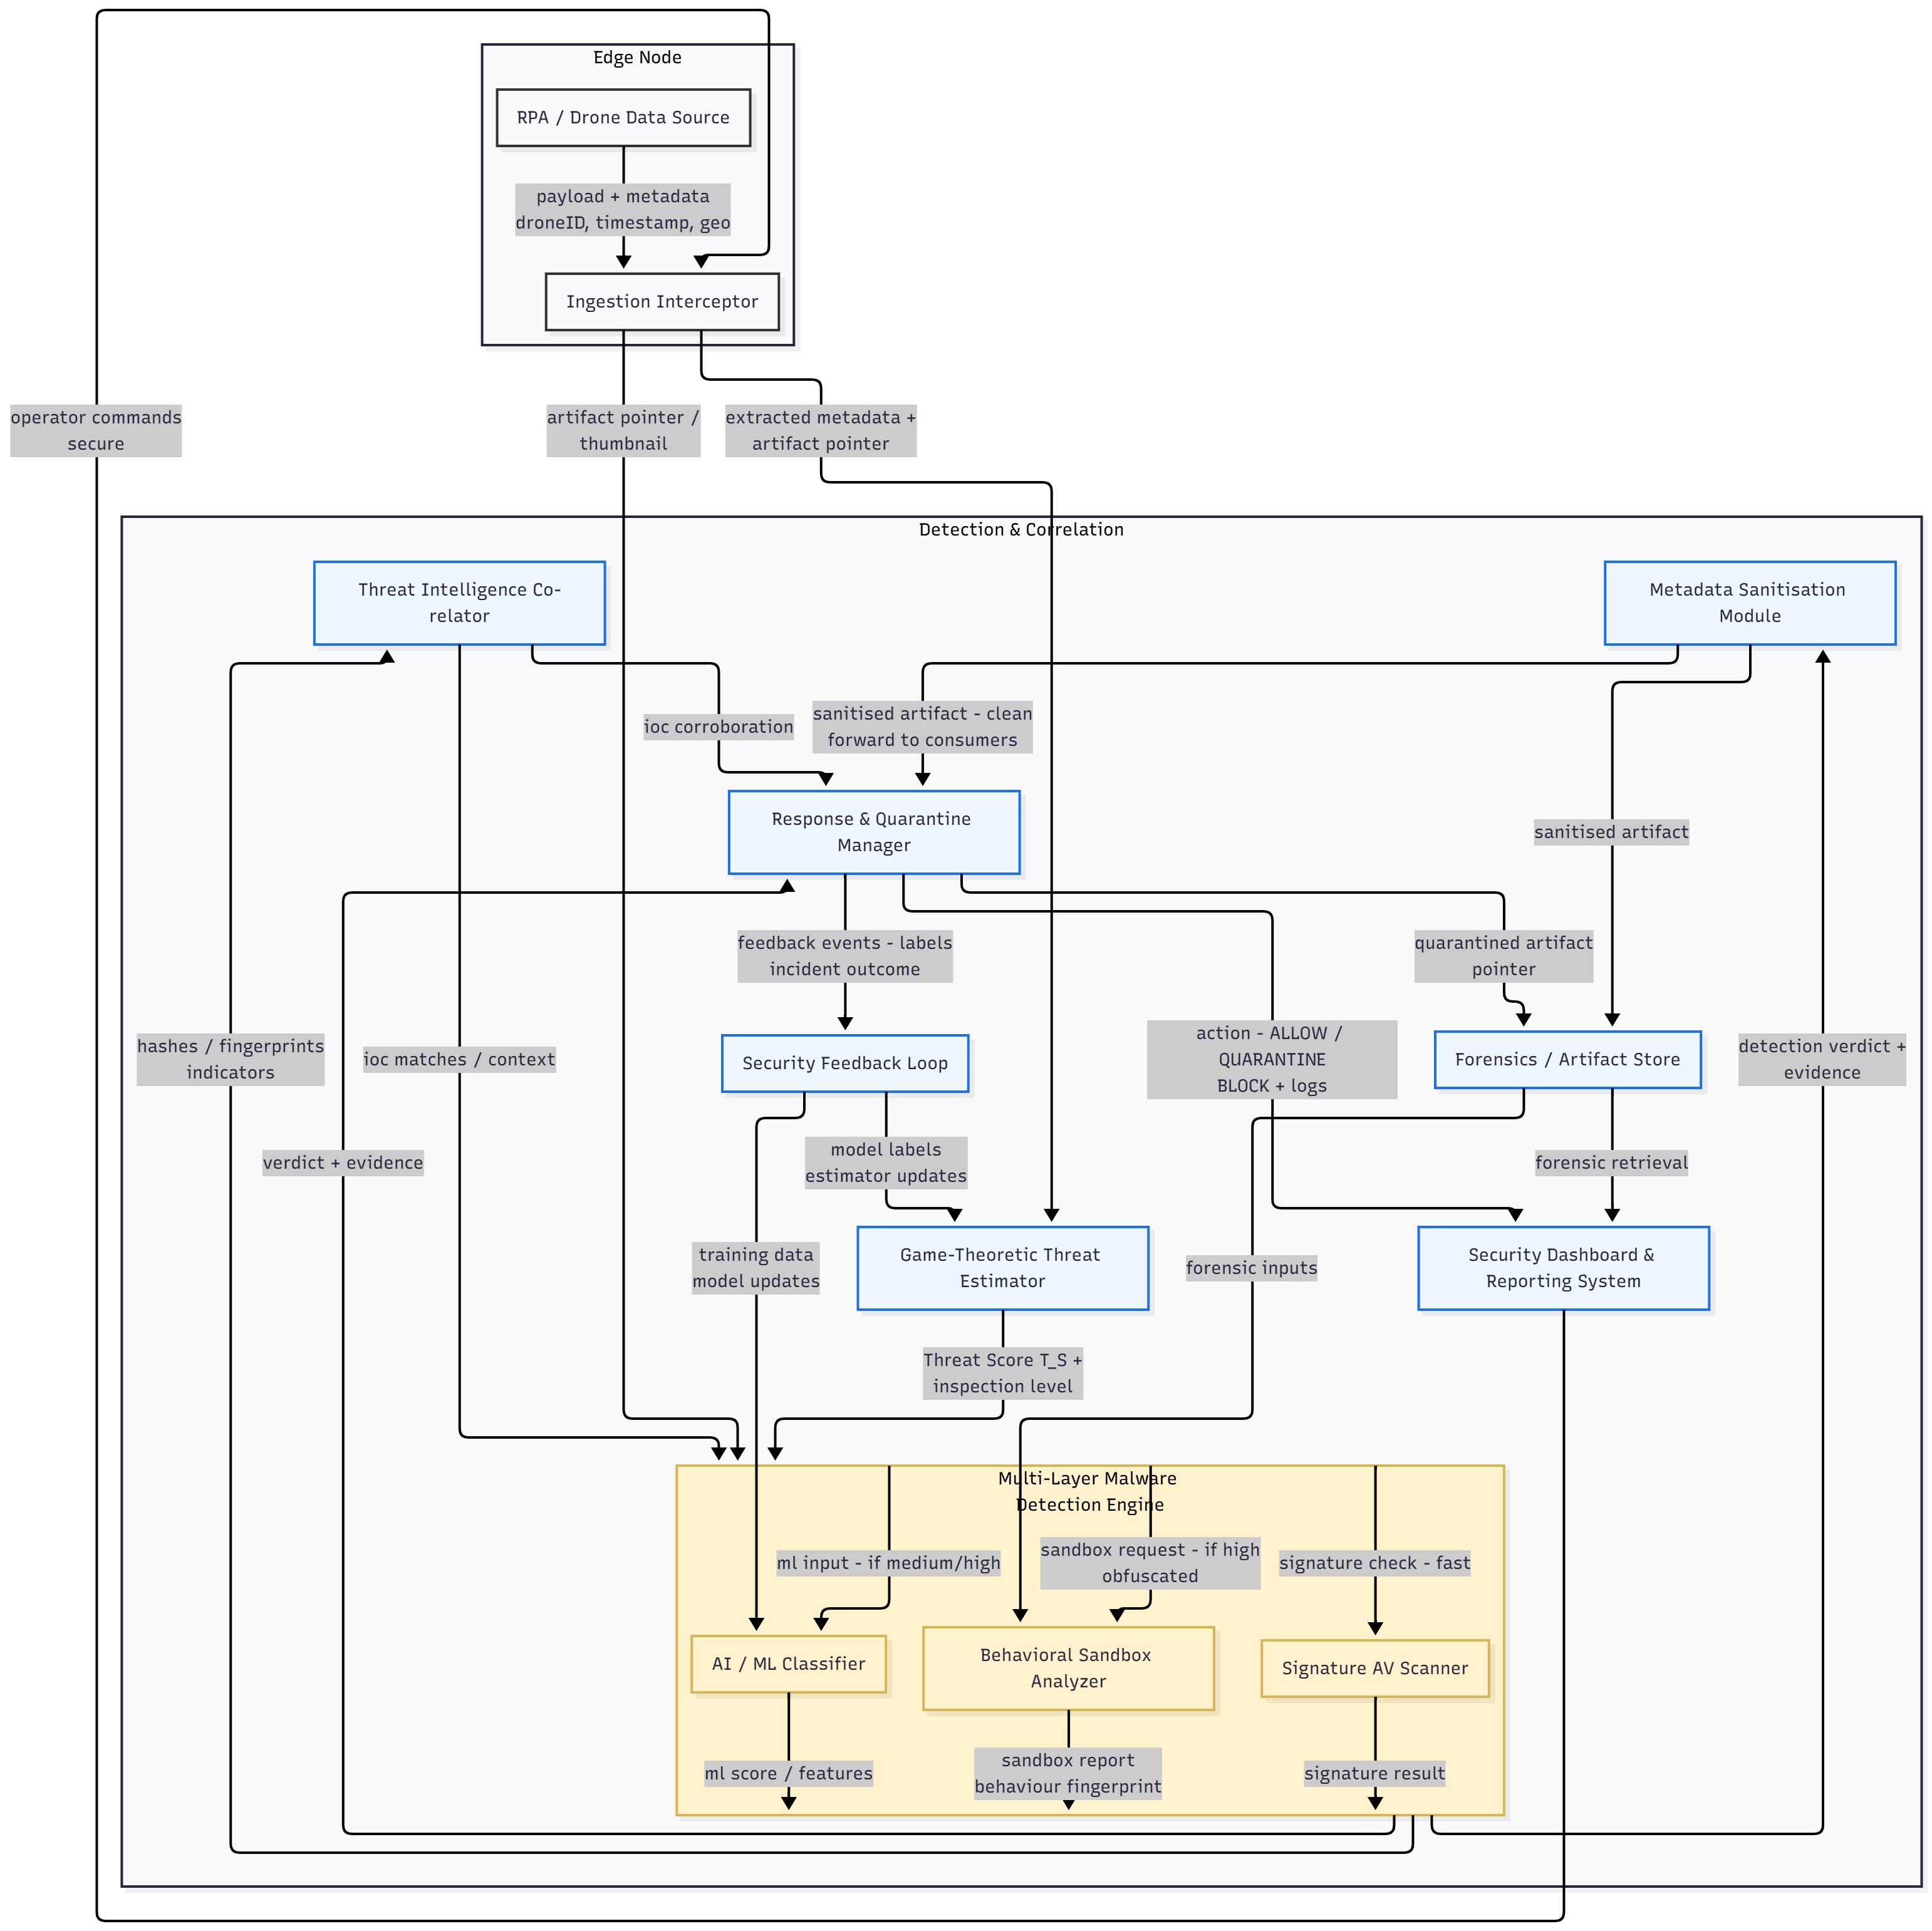
\includegraphics[width=\textwidth]{architecture_diagram.png}
    \caption{High-level architecture of the multi-layered malware detection
    pipeline.}
    \label{fig:system_overview}
\end{figure}

The major components are:
\begin{enumerate}
    \item \textbf{Drone / RPA Data Source} --- the origin of the data feed,
          consisting of video, images, encrypted or ZIP files, telemetry,
          text, and metadata.
    \item \textbf{Ingestion Interceptor} --- initial capture,
          authentication, and verification of incoming data streams.
          Implemented as part of this project
          (Chapter~\ref{chap:ingestion_interceptor}).
    \item \textbf{Game-Theoretic Threat Estimator} --- computes a numeric
          Threat Score ($T_S$) and selects the inspection depth.
          Implemented as part of this project (Chapter~\ref{chap:gte}).
    \item \textbf{Multi-Layer Malware Detection Engine} --- a progressive
          analysis stack activated based on the Threat Score:
          \begin{itemize}
              \item \emph{Signature-Based Malware Scanner} --- fast
                    detection of known malware through signature and IOC
                    matching (placeholder).
              \item \emph{AI/ML Malware Classifier} --- identifies
                    suspicious or malicious files that do not match known
                    signatures (placeholder).
              \item \emph{Sandbox Analyzer} --- deepest level of inspection
                    through isolated execution and kernel-level behavioural
                    observation. Implemented as part of this project
                    (Chapter~\ref{chap:sandbox}).
          \end{itemize}
    \item \textbf{Metadata Sanitizer} --- removes or normalises dangerous
          or hidden metadata fields before data is forwarded to consumers.
          Implemented as part of this project
          (Chapter~\ref{chap:metadata_sanitizer}).
    \item \textbf{Threat Intelligence Correlator} --- checks suspicious
          indicators against internal or external IOC feeds to confirm or
          enrich findings (placeholder; the Sandbox Analyzer already
          exposes a \texttt{ThreatIntelClient} seam that connects to it).
    \item \textbf{Response and Quarantine Manager} --- takes action based
          on detection results (allow, quarantine, block) (placeholder;
          receives verdicts through the Sandbox Analyzer's
          \texttt{FeedbackSink} seam).
    \item \textbf{Security Feedback Loop} --- closes the learning loop for
          adaptive defence. The Threat Estimator consumes the feedback
          loop's aggregated False Positive and False Negative Rates to
          soft-update its routing thresholds.
    \item \textbf{Security Dashboard and Reporting System} --- a
          centralised visibility and analytics interface (placeholder).
\end{enumerate}


\section{Data Flow Pipeline}

The end-to-end data flow pipeline is illustrated in
Figure~\ref{fig:data_flow} and summarised below.

\begin{figure}[H]
    \centering
    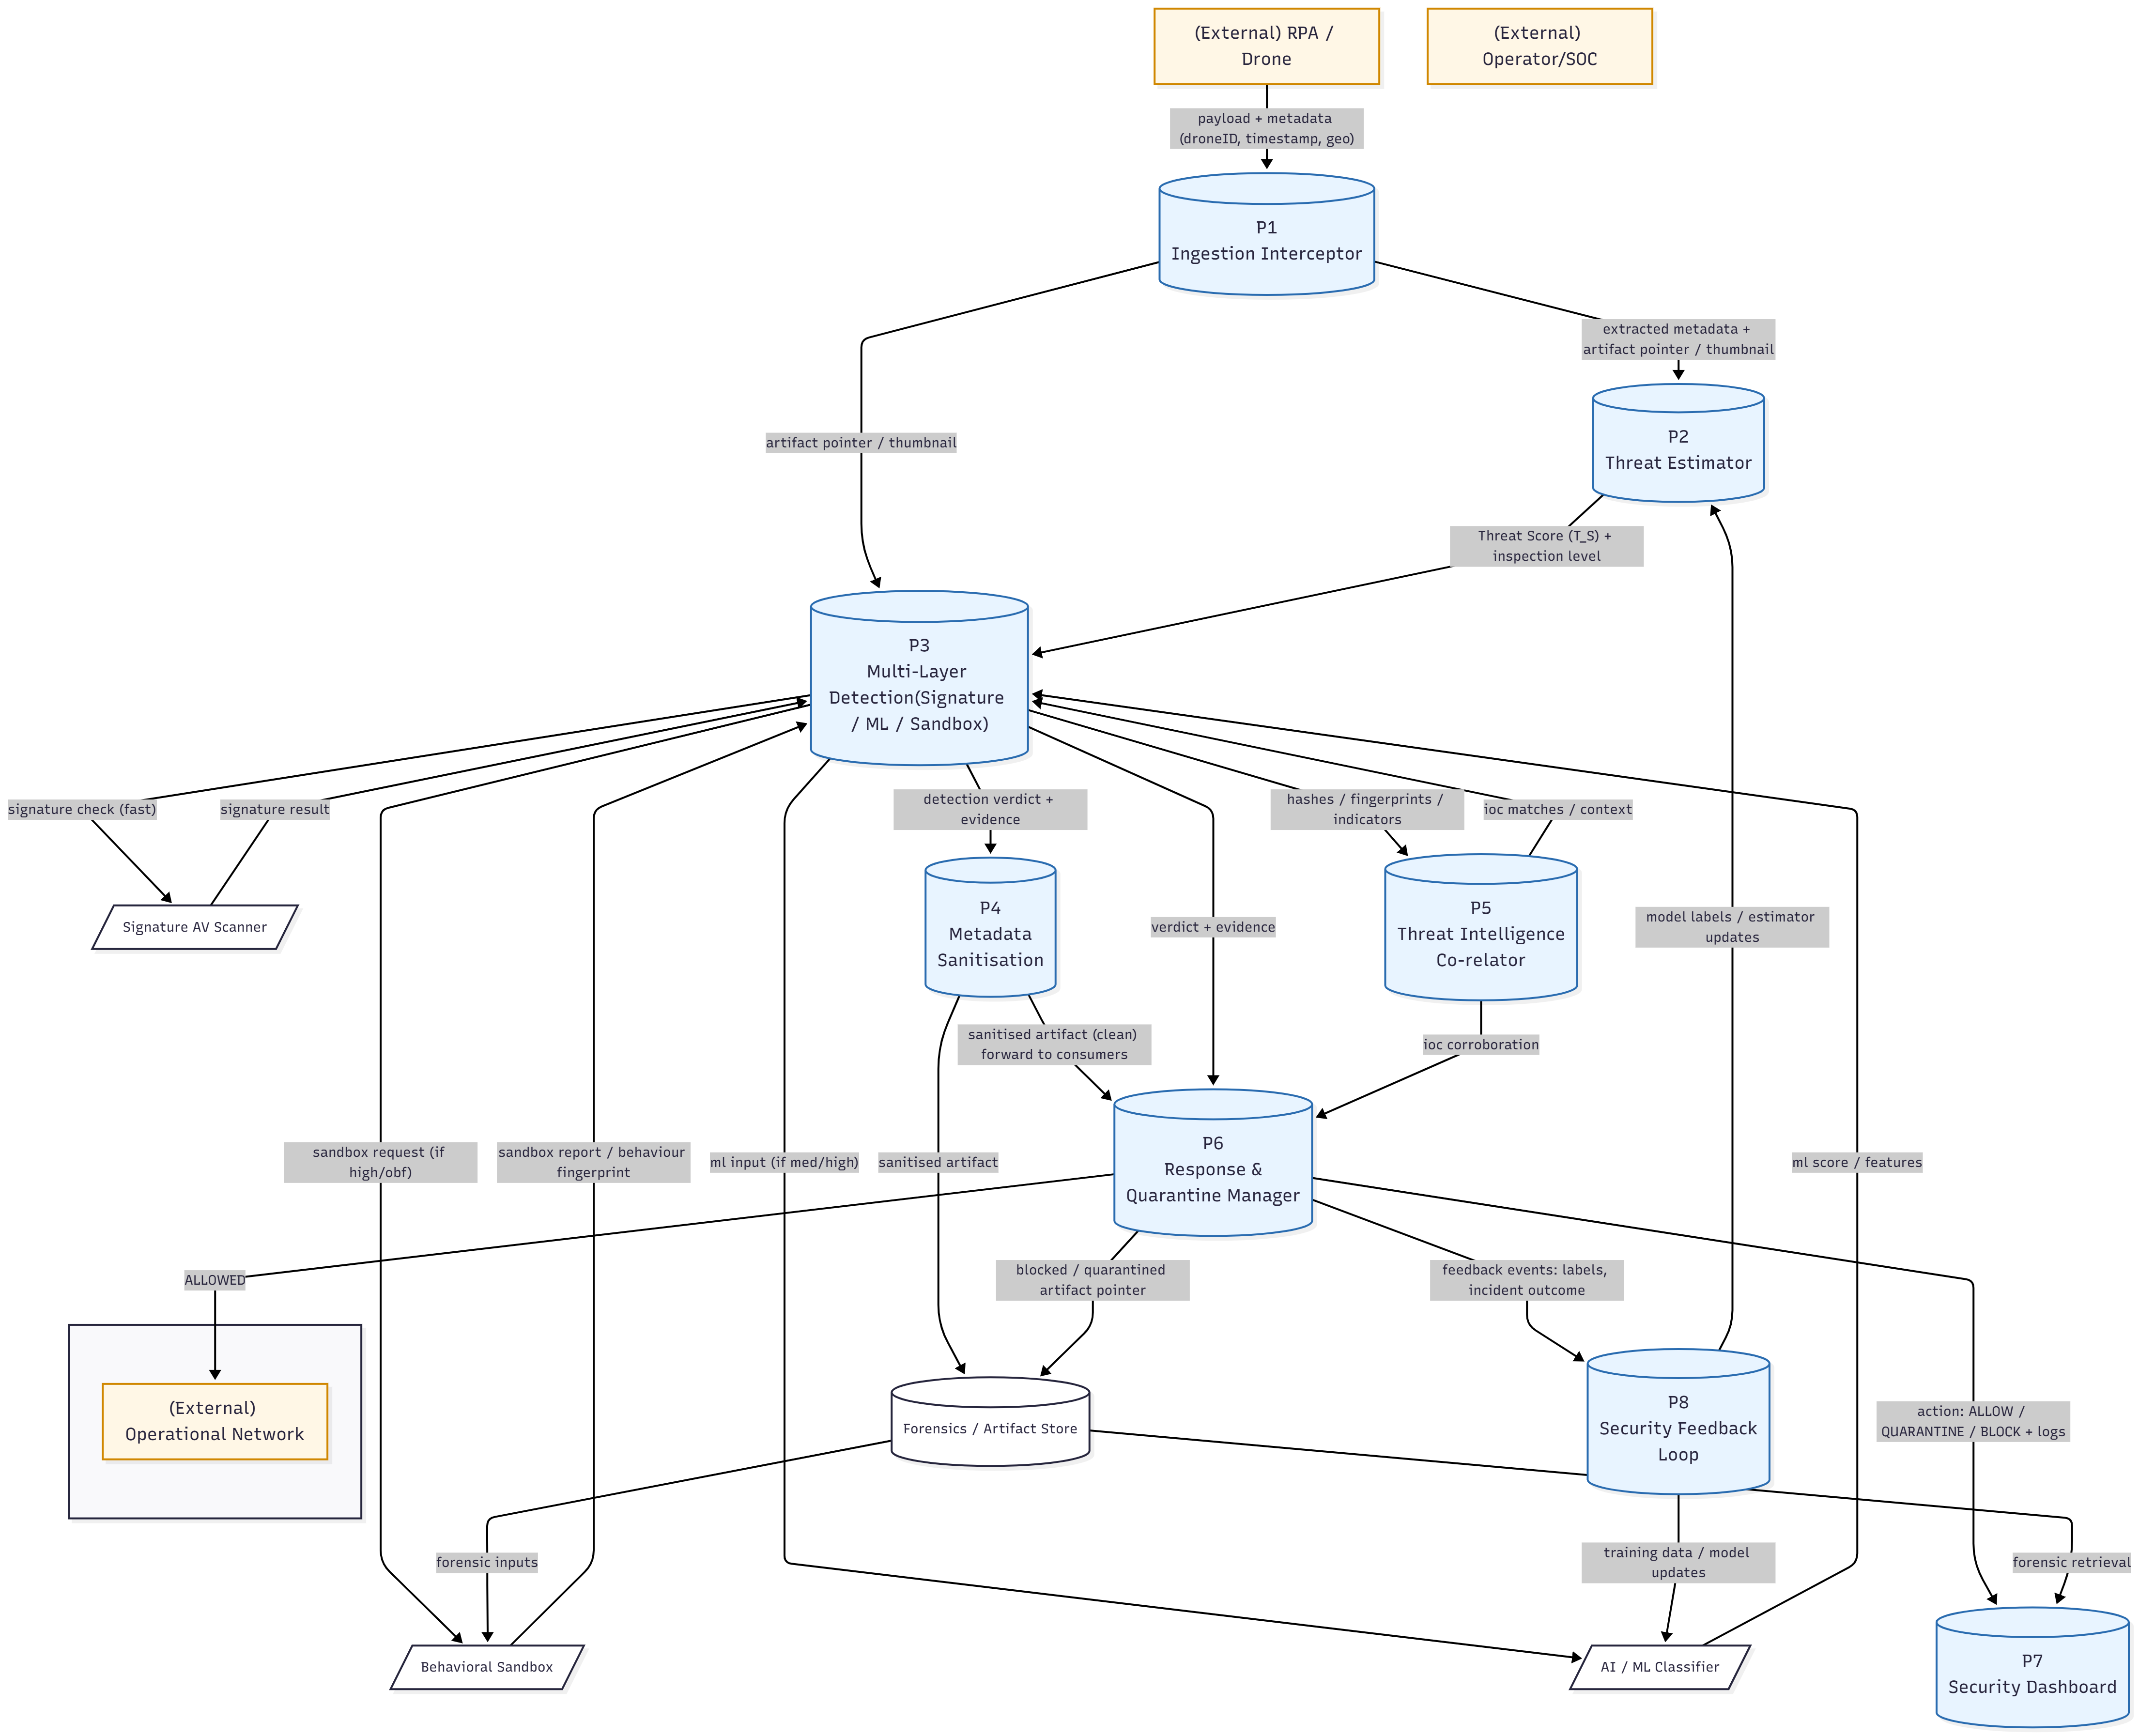
\includegraphics[width=0.95\textwidth]{data_flow_diagram.png}
    \caption{End-to-end data flow through the system.}
    \label{fig:data_flow}
\end{figure}

\begin{enumerate}
    \item \textbf{Drone transmits data.} The drone sends files or live
          streams along with metadata such as drone identifier, timestamp,
          geolocation, and mission zone.

    \item \textbf{Ingestion Interceptor captures data.} The interceptor
          receives and optionally reassembles UDP packets, authenticates
          the source, validates the submission, extracts metadata, flags
          insecure indicators, and produces a structured
          \texttt{IngestResult}.

    \item \textbf{Threat Estimator receives \texttt{IngestResult}.}
          The estimator consumes the interceptor's output and returns a
          Threat Score ($T_S$) together with an inspection decision
          (\emph{Low}, \emph{Medium}, or \emph{High}) and the ordered
          route of detection engines to invoke.

    \item \textbf{Detection engine applies layered inspection.} Depending
          on the inspection level:
          \begin{itemize}
              \item \emph{Low}: Signature scanner only.
              \item \emph{Medium}: Signature scanner and AI/ML classifier.
              \item \emph{High}: Signature scanner, AI/ML classifier, and
                    Sandbox Analyzer.
          \end{itemize}

    \item \textbf{Metadata sanitization.} The Metadata Sanitizer cleans
          embedded metadata. Its sanitization mode is selected
          automatically from the Threat Score: high scores trigger
          aggressive stripping, low scores default to audit-only logging.

    \item \textbf{Threat Intelligence correlation.} Hashes, IPs, and
          behavioural indicators are checked against known IOC feeds to
          reinforce or reduce detection confidence.

    \item \textbf{Response actions.} Based on the final verdict, the
          system allows, quarantines, or blocks the artifact and notifies
          operators.

    \item \textbf{Dashboard and operator interface.} Incidents are
          displayed on the dashboard. Operators may issue secure commands
          (quarantine, override inspection, etc.) which are forwarded back
          to the Ingestion Interceptor through its uplink channel.

    \item \textbf{Feedback loop.} Analyst-labelled samples and confirmed
          detections are aggregated into rolling False Positive and False
          Negative Rates that drive the Threat Estimator's adaptive
          thresholds and the Bayesian Conditional Probability Tables.
\end{enumerate}

\section{Cross-Module Interfaces}

The four implemented modules interact through well-defined typed data
structures rather than ad-hoc dictionaries. Table~\ref{tab:interfaces}
summarises the key interfaces.

\begin{table}[H]
\centering
\caption{Primary cross-module interfaces}
\label{tab:interfaces}
\begin{tabular}{|l|l|l|}
\hline
\textbf{Producer} & \textbf{Consumer} & \textbf{Interface} \\
\hline
Ingestion Interceptor & Threat Estimator & \texttt{IngestResult} dictionary \\
\hline
Threat Estimator & Detection Engine & Threat Score + inspection level \\
\hline
Threat Estimator & Metadata Sanitizer & Threat Score (selects mode) \\
\hline
Sandbox Analyzer & Response Manager & \texttt{SandboxReport} (verdict) \\
\hline
Sandbox Analyzer & Threat Intel Correlator & \texttt{ThreatIntelClient} seam \\
\hline
Response Manager & Threat Estimator & \texttt{DetectionOutcome} (feedback) \\
\hline
Feedback Loop & Threat Estimator & Rolling FPR / FNR metrics \\
\hline
\end{tabular}
\end{table}

\cleardoublepage


% ============================================================
% === CHAPTER 5: GAME-THEORETIC THREAT ESTIMATOR ============
% ============================================================

\chapter{Game-Theoretic Threat Estimator}
\label{chap:gte}

\section{Introduction}

Multi-layer malware detection pipelines typically combine several analysis
stages: ingestion filters, static scanners, machine learning classifiers and
sandbox-based behavioural engines. Each stage produces partial and sometimes
noisy evidence, and it is not obvious how to convert this heterogeneous
information into a single, interpretable \textbf{Threat Score}.

The \textbf{Game-Theoretic Threat Estimator (GTE)} developed in this project
provides a lightweight, mathematically principled way to fuse ingestion-level
evidence into a continuous risk score $T_S \in [0,1]$. The estimator is
inspired by attacker--defender utility models:

\begin{itemize}
    \item the \textbf{attacker} strategically chooses concealment techniques
          such as encryption or nested archives;
    \item the \textbf{defender} chooses the inspection depth under
          computational and time constraints.
\end{itemize}

Instead of solving a full dynamic game, the implemented GTE uses
\emph{game-theoretic ideas} (utility, advantage, monotonic risk aggregation)
in a form that is simple enough to deploy on edge hardware. It operates
directly on the structured outputs produced by the Ingestion Interceptor.


\section{Game Theoretic Threat Estimator Core}

At the heart of the system, the Game-Theoretic Threat Estimator models a
two-player game between a defender and an adversary:

\begin{itemize}
    \item The \textbf{Defender (System)} chooses the \emph{inspection depth}.
    \item The \textbf{Attacker (Adversary)} chooses the \emph{attack strength}.
\end{itemize}

Table~\ref{tab:gte-core-roles} summarises the roles and choices.

\begin{table}[H]
\centering
\caption{Core roles and choices in the game-theoretic model}
\label{tab:gte-core-roles}
\begin{tabular}{|l|l|p{6cm}|}
\hline
\textbf{Role} & \textbf{Player} & \textbf{Choices} \\
\hline
Defender (System) &
Chooses inspection depth &
Signature, AI/ML, Sandbox \\
\hline
Attacker (Adversary) &
Chooses attack strength &
No attack, simple malware, obfuscated malware \\
\hline
\end{tabular}
\end{table}

The estimator predicts how smart or aggressive the attacker might be and then
selects the most cost-effective defence strategy, balancing detection strength
against computational and latency costs.
\subsection*{The Reasoning Behind It}



\begin{itemize}
    \item Each defense has a cost (CPU time, latency).
    \item Each attack has a gain or loss depending on whether it succeeds or fails.
    \item The estimator simulates both sides, calculates possible outcomes, and decides the best defense level that minimizes overall risk.

\end{itemize}

Through these reasonings, the estimator selects the inspection depth that \textbf{minimizes overall system risk} while avoiding unnecessary high-cost analysis.

\section{Game Mathematics in Simple Terms}

In the Game-Theoretic Threat Estimator, every interaction between the defender’s inspection strategy and the attacker’s chosen action can be represented through payoff outcomes. Each pair of choices produces different costs, risks, and expected gains.

\subsection*{Strategy Interaction Overview}

\begin{table}[h!]
\centering
\begin{tabular}{|c|c|c|}
\hline
\textbf{Defender Strategy} & \textbf{No Attack} & \textbf{Attack} \\ \hline
Signature Scan & Low cost, low catch rate & Cheap but risky \\ \hline
AI/ML Scan & Moderate cost, better detection & Balanced outcome \\ \hline
Sandbox & Expensive, strong catch capability & High cost but safest \\ \hline
\end{tabular}
\end{table}

\subsection*{Utility Formulation}

The system models both sides using utility functions:

\begin{itemize}
    \item \textbf{Defender Utility}:
    \[
        U_d = \text{benefit of detection} - \text{inspection cost}
    \]

    \item \textbf{Attacker Utility}:
    \[
        U_a = \text{successful impact of attack} - \text{effort/cost of attack}
    \]
\end{itemize}

\subsection*{Equilibrium Selection}

The estimator evaluates all possible combinations of actions by both players and computes the \textbf{Stackelberg equilibrium}.  

This equilibrium represents:

\begin{quote}
\textit{The defender’s optimal inspection strategy, assuming the attacker responds in the most advantageous way for themselves.}
\end{quote}

Thus, the chosen inspection level is both rational and cost-effective, minimizing risk while avoiding unnecessary computational overhead.


\section{Parameters That Influence the Game}

\begin{table}[h!]
\centering
\begin{tabular}{|c|c|c|}
\hline
\textbf{Parameter} & \textbf{Meaning} & \textbf{Example} \\ \hline
$R$ & Reputation of drone (trust) & Based on history, 0--1 \\ \hline
$Z$ & Zone risk & 0 = safe base, 1 = warzone \\ \hline
$H$ & Past infection rate & Higher $\rightarrow$ more suspicious \\ \hline
$I_{\text{base}}$ & Impact of file type & Images = low, encrypted ZIPs = high \\ \hline
$C_d$ & Defender cost per strategy & Sandbox costs more than signature \\ \hline
$DSR$ & Detection success rate & How effective each layer is \\ \hline
$T_S$ & Threat score & Final 0--1 score derived from the equilibrium \\ \hline
\end{tabular}
\end{table}

\noindent NOTE: More parameters may be added in future.

\section{Outcome}

The estimator produces two outputs:

\begin{verbatim}
{
  "Threat_Score": 0.72,
  "Inspection_Level": "High"
}
\end{verbatim}

If $T_S < 0.4$ → Low (Signature only)

If $0.4 \leq T_S < 0.7$ → Medium (Signature + ML)

If $T_S \geq 0.7$ → High (Sandbox)

\subsection*{Intuitive Example}

\begin{table}[h!]
\centering
\begin{tabular}{|c|c|c|c|c|c|}
\hline
\textbf{Drone ID} & \textbf{Reputation} & \textbf{Zone Risk} & \textbf{Past Infection} & \textbf{Threat Score} & \textbf{Decision} \\ \hline
DRN-001 & 0.9 & 0.2 & 0.0 & 0.25 & Low (Signature) \\ \hline
DRN-007 & 0.6 & 0.7 & 0.3 & 0.65 & Medium (ML) \\ \hline
DRN-013 & 0.3 & 0.8 & 0.6 & 0.85 & High (Sandbox) \\ \hline
\end{tabular}
\end{table}


\section{Variables, Inputs \& Assumptions}

These are the variables and parameters required by the estimator for each incoming artifact. Use these exact names in code and notebooks.

\subsection*{Core Inputs from the Ingestion Interceptor}

\begin{itemize}
    \item \texttt{drone\_id} — string. Unique ID for the sending drone.
    \item \texttt{timestamp} — ISO8601 string. When the feed was captured.
    \item \texttt{mission\_zone} — string. Named area or zone id (used to look up zone risk).
    \item \texttt{geo} — object \{lat, lon, alt\}. (optional for now)
    \item \texttt{artifact\_records} — list of artifacts (each with: filename, type, mime, size\_bytes, encryption, container, checksum, thumbnail, pointer\_storage).
\end{itemize}

\subsection*{Derived / System Inputs (lookup or compute at estimator)}

\begin{itemize}
    \item $R$ — reputation of the drone/source, numeric in [0, 1].  
    1 = fully trusted, 0 = fully untrusted.  
    Default: 0.8 for new devices.  
    Source: reputation DB (Redis/Postgres) updated by Feedback Loop.

    \item $Z$ — zone risk, numeric in [0, 1].  
    0 = safe zone, 1 = highest-risk (e.g., conflict area).  
    Default: 0.5 (neutral) if unknown.  
    Source: static policy table or dynamic intelligence.

    \item $H$ — recent infection frequency for this drone (or zone), numeric in [0, 1].  
    Fraction of recent feeds confirmed malicious.  
    Default: 0.0 if no historic detections.  
    Example: 0.2 means 20\% of last N feeds were malicious.

    \item \texttt{TI\_boost} — threat-intel corroboration strength, numeric in [0, 1].  
    0 if no IOC matches; \(>0\) if indicators match known bad IOCs.  
    Default: 0.0.

    \item $I_{\text{base}}$ — base impact of the artifact (0..10).  
    How bad it would be if this artifact were malicious.  
    Example mapping:  
    telemetry/small text → 1–2  
    images → 3–6  
    video/large survey → 6–9  
    encrypted archive → 8–10  
    Default: compute from \texttt{artifact\_records}.
\end{itemize}

\subsection*{Defender / Attacker Model Constants (tunable)}

\begin{itemize}
    \item $DSR(s)$ — base detection success rate per defender strategy, value in (0,1).  
    Defaults:  
    DSR('signature') = 0.70  
    DSR('ml') = 0.85  
    DSR('sandbox') = 0.95

    \item $C_d(s)$ — defender cost for strategy s.  
    Defaults:  
    C\_d('signature') = 1.0  
    C\_d('ml') = 3.0  
    C\_d('sandbox') = 6.0

    \item $C_a(a)$ — attacker cost for action a.  
    Defaults:  
    C\_a('inject') = 2.0  
    C\_a('no\_inject') = 0.0
\end{itemize}

\subsection*{Tunable Weights and Small Constants}

\begin{itemize}
    \item $\alpha$ — reputation influence on impact (default 0.5).
    \item $\beta$ — zone risk influence on impact (default 0.3).
    \item $\gamma$ — history effect on detection (default 0.2).
    \item $\delta$ — TI boost effect on detection (default 0.0).
    \item $\kappa$ — sigmoid scale for raw → normalized mapping (default 0.8).
    \item $\lambda_{\text{blend}}$ — blend weight for model score and reputation (default 0.9).
    \item $\varepsilon$ — clamp epsilon (default 0.001).
\end{itemize}

\subsection*{Thresholds — Inspection Mapping}

\begin{itemize}
    \item \texttt{th\_low} = 0.4
    \item \texttt{th\_high} = 0.7
\end{itemize}


\section{Bayesian Cold-Start Reputation}
\label{sec:gte-bayes}

\subsection{Motivation}

When a brand-new drone enters the network, it has no history in the
reputation database. Assigning a static default reputation is dangerous:
a sophisticated adversary could spin up a new drone identity and exploit
a permissive default to bypass deep inspection.

The GTE solves this cold-start problem using observable context. Two
context attributes are always known at the ingestion point:
\begin{itemize}
    \item the operational zone ($Z$);
    \item the dominant file type ($F$) of the submission.
\end{itemize}

These two attributes, combined with a prior on benign traffic, are
enough to compute a principled initial reputation.

\subsection{Bayesian Belief Network}

Figure~\ref{fig:bbn-topology} shows the topology of the belief network
used. The attack status (\emph{Benign} or \emph{Malicious}) is the
unobserved variable; the zone and file type are observed.

\begin{figure}[H]
\centering
\fbox{\begin{minipage}{0.65\linewidth}
\begin{center}
Zone ($Z$) \quad\quad\quad\quad File Type ($F$) \\[0.3em]
$\searrow$\hspace{2em}$\swarrow$ \\[0.2em]
Attack Status $\in \{\text{Benign}, \text{Malicious}\}$
\end{center}
\end{minipage}}
\caption{Bayesian Belief Network used for cold-start reputation.
Observed evidence ($Z$ and $F$) influences the unobserved attack status;
conditional independence is assumed between $Z$ and $F$ given the attack
status.}
\label{fig:bbn-topology}
\end{figure}

\subsection{Posterior Formulation}

Let $N$ denote \emph{No Attack (Benign)} and $A$ denote \emph{Attack
(Malicious)}. The reputation is the posterior probability of the benign
class given the observed context:

\[
R = P(N \mid Z, F) = \frac{P(N) \, P(Z \mid N) \, P(F \mid N)}
{P(N) \, P(Z \mid N) \, P(F \mid N) + P(A) \, P(Z \mid A) \, P(F \mid A)}.
\]

The priors $P(N)$ and $P(A) = 1 - P(N)$ and the likelihoods
$P(Z \mid \cdot)$ and $P(F \mid \cdot)$ are stored in Conditional
Probability Tables (CPTs). The CPTs are seeded with expert values and
refreshed by the feedback loop as labelled detections accumulate.

\subsection{Worked Example}

Consider a drone submitting a ZIP file from a risky zone. With a benign
prior of $0.85$, the CPT entries might be:
\begin{itemize}
    \item $P(Z = \text{zone-3} \mid N) = 0.12$, $P(Z = \text{zone-3} \mid A) = 0.35$;
    \item $P(F = \text{zip} \mid N) = 0.08$, $P(F = \text{zip} \mid A) = 0.45$.
\end{itemize}

Plugging into Bayes' rule:
\[
\text{numerator} = 0.85 \times 0.12 \times 0.08 = 0.00816,
\]
\[
\text{denominator} = 0.00816 + (0.15 \times 0.35 \times 0.45) = 0.031785,
\]
\[
R \approx 0.257.
\]

A reputation of $0.257$ correctly flags this previously unseen submission
as moderately suspicious and pushes it toward deeper inspection in the
subsequent stages.


\section{Compute Adjusted Parameters ($I'$, DSR$'(s)$)}

We compute two quantities required before building payoff matrices:

\begin{itemize}
    \item \textbf{Adjusted impact} ($I'$) — how bad it is if an artifact is malicious, after accounting for reputation and zone risk.
    \item \textbf{Adjusted detection success rates} (DSR$'(s)$) — how likely each defense is to catch malware given history and TI.
\end{itemize}

\subsection{Formula: Adjusted impact ($I'$)}

\[
I' = I_{\text{base}} \, (1 + \alpha (1 - R)) \, (1 + \beta Z)
\]

\subsubsection*{Terms explained}

\begin{itemize}
    \item $I_{\text{base}}$: base impact (0--10), derived from file type / mission sensitivity.
    \item $R$ (0--1): reputation (1 = trusted). The factor $(1-R)$ increases impact if reputation is low.
    \item $\alpha$: influence of reputation on impact (default 0.5).
    \item $Z$ (0--1): zone risk.
    \item $\beta$: influence of zone risk on impact (default 0.3).
\end{itemize}

\subsubsection*{Why multiplicative?}

Multiplying keeps effects proportional — a high base impact in a risky zone with low reputation becomes substantially larger.

\subsubsection*{Defaults}

(As defined earlier.)

\subsubsection*{Heuristic for $I_{\text{base}}$}

Estimate from artifact types and sizes:

\begin{table}[h!]
\centering
\begin{tabular}{|c|c|}
\hline
Type & Typical $I_{\text{base}}$ \\ \hline
telemetry / small text & 1--2 \\ \hline
image & 3--6 \\ \hline
video / survey & 6--9 \\ \hline
encrypted archive / executable & 8--10 \\ \hline
\end{tabular}
\end{table}

Example heuristic formula:

\[
I_{\text{base}} = \mathrm{clip}\big( 3 + 3 \cdot \text{avg\_size\_MB} + 3 \cdot \text{type\_risk},\ 0,\ 10 \big)
\]

where type\_risk = 0.2 / 0.7 / 0.9 for low / archive / video.


\subsection{Formula: Adjusted detection success rate (DSR$'(s)$)}

\[
\mathrm{DSR}'(s) =
\mathrm{clamp}\Big( \mathrm{DSR}(s)\,(1 - \gamma H)\,(1 + \delta\,\mathrm{TI}),\ \varepsilon,\ 1 - \varepsilon \Big)
\]

where $\mathrm{clamp}(x,a,b)=\max(a,\min(b,x))$.

\subsubsection*{Terms explained}

\begin{itemize}
    \item $\mathrm{DSR}(s)$: base detection success rate (signature/ml/sandbox).  
          Defaults: 0.70 / 0.85 / 0.95.
    \item $H$ (0--1): recent infection frequency. Factor $(1-\gamma H)$ reduces DSR.
    \item $\gamma$: history effect (default 0.2).
    \item TI (0--1): threat-intel corroboration strength.
    \item $\delta$: TI multiplier (default 0.0).
    \item $\varepsilon$: clamp epsilon (default 0.001).
\end{itemize}

\subsubsection*{Why multiplicative?}

History degrades success proportionally (e.g., 0.90 → 0.80).  
TI slightly boosts DSR when relevant.



\section{Payoff Matrices and Utilities}

\subsection*{Recap of Inputs}

From previous steps, the following inputs are available:

\begin{itemize}
    \item Adjusted impact $I'$ (scalar)
    \item Adjusted detection success rates $\mathrm{DSR}'(s)$
    \item Defender cost per strategy $C_d(s)$
    \item Attacker cost per action $C_a(a)$
\end{itemize}

Defender strategies:
\[
S_d = \{\text{signature},\ \text{ml},\ \text{sandbox}\}
\]

Attacker actions:
\[
S_a = \{\text{inject},\ \text{no\_inject}\}
\]

These inputs form two matrices:

\begin{itemize}
    \item $U_d(i,j)$: defender payoff when defender selects strategy $i$ and attacker selects action $j$
    \item $U_a(i,j)$: attacker payoff for the same cell
\end{itemize}

Rows correspond to defender strategies, columns to attacker actions.

\subsection*{Payoff Formulas}

\paragraph{Defender payoff}
\[
U_d(s,a)=
\begin{cases}
\mathrm{DSR}'(s)\, I' - C_d(s), & a=\text{inject} \\
-C_d(s), & a=\text{no\_inject}
\end{cases}
\]

Interpretation:
\begin{itemize}
    \item If attacker injects → defender gains expected prevented impact minus inspection cost.
    \item If attacker does not inject → defender only pays inspection cost.
\end{itemize}

\paragraph{Attacker payoff}
\[
U_a(s,a)=
\begin{cases}
(1-\mathrm{DSR}'(s))\, I' - C_a(a), & a=\text{inject} \\
0, & a=\text{no\_inject}
\end{cases}
\]

Interpretation:
\begin{itemize}
    \item Expected successful impact $(\text{ASP} \times I')$ minus attacker cost.
    \item If no injection → payoff = 0.
\end{itemize}

\subsection*{Matrix Layout}

\paragraph{Attacker Utility Matrix}
\begin{table}[H]
\centering
\begin{tabular}{|l|c|c|}
\hline
 & inject & no\_inject \\
\hline
signature & $U_a(\text{sig},\text{inject})$ & 0 \\
\hline
ml & $U_a(\text{ml},\text{inject})$ & 0 \\
\hline
sandbox & $U_a(\text{sbx},\text{inject})$ & 0 \\
\hline
\end{tabular}
\end{table}

\paragraph{Defender Utility Matrix}
\begin{table}[H]
\centering
\begin{tabular}{|l|c|c|}
\hline
 & inject & no\_inject \\
\hline
signature & $U_d(\text{sig},\text{inject})$ & $-C_d(\text{sig})$ \\
\hline
ml & $U_d(\text{ml},\text{inject})$ & $-C_d(\text{ml})$ \\
\hline
sandbox & $U_d(\text{sbx},\text{inject})$ & $-C_d(\text{sandbox})$ \\
\hline
\end{tabular}
\end{table}

Both matrices are computed and logged for audit.

\subsection*{Decision Logic (Stackelberg Pure-Strategy Enumerator)}

Defender acts as the leader:

\begin{enumerate}
    \item For each defender strategy $s$:
    \begin{enumerate}
        \item Attacker selects best response $a^*(s)$
        \item Defender evaluates resulting payoff $U_d(s,a^*(s))$
    \end{enumerate}
    \item Defender selects strategy
    \[
    s^* = \arg\max_s U_d(s,a^*(s))
    \]
    \item Equilibrium cell:
    \[
    (s^*, a^*(s^*))
    \]
\end{enumerate}

Tie-breaking:
\begin{itemize}
    \item Attacker prefers the action that harms defender more.
    \item Defender prefers the cheaper strategy among equal payoffs.
\end{itemize}

Overall complexity: $O(|S_d|\cdot|S_a|)$.

\section{From Equilibrium Utilities to Threat Score and Inspection Level}

We now convert the equilibrium utilities computed in the previous step into a
single, bounded Threat Score and an actionable inspection level. The process is:
compute a raw attacker–defender advantage, normalize it with a sigmoid,
blend it with reputation, apply thresholds to derive the inspection level, and
use a worked numeric example.

\subsection*{Why This Mapping and Goals}

Raw utilities $U_a^{\text{eq}}$ and $U_d^{\text{eq}}$ are in abstract units and can be
negative or large. We need a compact value in $[0,1]$ to:

\begin{itemize}
    \item route inspection decisions, and
    \item monitor behaviour over time.
\end{itemize}

The mapping should reflect attacker advantage:

\begin{itemize}
    \item if attacker utility $>$ defender utility, threat should be higher;
    \item we also want reputation to reduce risk for known-good sources.
\end{itemize}

\subsection*{Step A — Raw Metric}

Compute the attacker advantage as:
\[
\text{raw} = U_a^{\text{eq}} - U_d^{\text{eq}}.
\]

\begin{itemize}
    \item If $\text{raw} > 0$, attacker is ahead $\Rightarrow$ worry more.
    \item If $\text{raw} < 0$, defender is ahead $\Rightarrow$ less worry.
\end{itemize}

\subsection*{Step B — Sigmoid Normalization}

Map \texttt{raw} to a $[0,1]$ value using a sigmoid function:
\[
T_{\text{raw}} = \frac{1}{1 + e^{-\kappa \cdot \text{raw}}}
\]
where $\kappa$ controls sensitivity (default $\kappa = 0.8$).

\begin{itemize}
    \item Larger $\kappa$ makes the sigmoid steeper (small raw differences
          produce larger changes in $T_{\text{raw}}$).
    \item Smaller $\kappa$ smooths differences.
\end{itemize}

\subsection*{Step C — Blend with Reputation Prior}

Blend the model signal with the reputation prior so trusted sources are penalised
less:
\[
T_S = \lambda_{\text{blend}} \, T_{\text{raw}} + (1 - \lambda_{\text{blend}})\,(1 - R),
\]
where:
\begin{itemize}
    \item $\lambda_{\text{blend}}$ (default $0.9$) controls how much weight the
          model output gets versus the reputation prior,
    \item $R$ is the reputation in $[0,1]$.
\end{itemize}

Then clamp to $[\varepsilon, 1 - \varepsilon]$:
\[
T_S \leftarrow \mathrm{clamp}(T_S,\ \varepsilon,\ 1-\varepsilon)
\]
with a small $\varepsilon$ (e.g., $\varepsilon = 0.001$).

Here $T_S$ is the final threat probability-like score.

\subsection*{Step D — Map $T_S$ to Inspection Level}

Use thresholds to select inspection depth. With default thresholds:
\[
\text{th}_{\text{low}} = 0.4, \qquad \text{th}_{\text{high}} = 0.7,
\]
the mapping is:

\begin{itemize}
    \item Low: $T_S < \text{th}_{\text{low}}$  
          $\Rightarrow$ Signature only
    \item Medium: $\text{th}_{\text{low}} \le T_S < \text{th}_{\text{high}}$  
          $\Rightarrow$ Signature + ML
    \item High: $T_S \ge \text{th}_{\text{high}}$  
          $\Rightarrow$ Signature + ML + Sandbox
\end{itemize}



\section{Reputation Dynamics}

Once a detection verdict is available, the reputation is updated using
an asymmetric reward--penalty rule:

\[
R_{\text{new}} =
\begin{cases}
\text{clip}(R + \eta_+ (1 - R), 0, 1) & \text{if verdict is benign}, \\
\text{clip}(R - \eta_- R, 0, 1) & \text{if verdict is malicious}, \\
R & \text{otherwise (unknown / quarantined)}.
\end{cases}
\]

With default rates $\eta_+ = 0.05$ (reward) and $\eta_- = 0.50$
(penalty), a single confirmed infection halves a drone's reputation,
while recovery requires many successive benign verdicts. The asymmetry
reflects the operational cost of false negatives in a
security-critical setting.

When a cold-start drone receives its first verdict, the update is
seeded from the Bayesian prior rather than from the generic default,
so the context-derived reputation is not discarded by the first
feedback event.


\section{Adaptive Threshold Manager}

Static thresholds become sub-optimal as attack patterns drift. The GTE
addresses this with an \textbf{Adaptive Threshold Manager} that
soft-updates $\theta_{\text{low}}$ and $\theta_{\text{high}}$ based on
observed False Positive Rate (FPR) and False Negative Rate (FNR).

The update rule for a monitoring window is:
\[
\theta_{\text{new}} = \theta_{\text{old}} + \eta \, (\mathrm{FPR} - \mathrm{FPR}_{\text{target}})
- \eta \, (\mathrm{FNR} - \mathrm{FNR}_{\text{target}}),
\]
where $\eta$ is a small learning rate. Intuitively:
\begin{itemize}
    \item when FPR is above target, thresholds rise so that fewer
          submissions are escalated to the expensive deep inspection
          layers;
    \item when FNR is above target, thresholds fall so that more
          submissions receive deeper inspection and evasions are less
          likely.
\end{itemize}

After each update, the thresholds are clamped to configurable safe
bounds (for example,
$\theta_{\text{low}} \in [0.20, 0.50]$ and
$\theta_{\text{high}} \in [0.55, 0.85]$), and a minimum gap between
them is enforced so that the band never collapses. Disabling the
adaptive behaviour is a configuration flag for deterministic replays
and controlled comparisons.


\section{Feedback Loop}

The GTE's feedback loop aggregates detection verdicts into rolling
FPR and FNR metrics over a bounded window. The accounting rule is:
\begin{itemize}
    \item \emph{High} or \emph{Medium} inspection followed by a
          \emph{malicious} verdict counts as a True Positive;
    \item \emph{High} or \emph{Medium} inspection followed by a
          \emph{benign} verdict counts as a False Positive;
    \item \emph{Low} inspection followed by a \emph{malicious} verdict
          counts as a False Negative;
    \item \emph{Low} inspection followed by a \emph{benign} verdict
          counts as a True Negative;
    \item \emph{unknown} or \emph{quarantined} verdicts are ignored.
\end{itemize}

The host process calls \texttt{record\_outcome()} after every verdict
and periodically calls \texttt{update\_thresholds\_from\_feedback()} to
let the manager pick up the latest metrics.


\section{Configuration and Defaults}
\label{sec:gte-config}

Table~\ref{tab:gte-defaults} lists the default values of the most
operationally relevant parameters. All values are tunable through the
\texttt{EstimatorConfig} dataclass, whose \texttt{\_\_post\_init\_\_}
method rejects any inconsistent combination at construction time.

\begin{table}[H]
\centering
\caption{GTE default configuration values}
\label{tab:gte-defaults}
\begin{tabular}{|p{5.2cm}|c|p{5.8cm}|}
\hline
\textbf{Parameter} & \textbf{Default} & \textbf{Meaning} \\
\hline
$\alpha$ & $0.5$ & reputation weight on $I'$ \\
\hline
$\beta$ & $0.3$ & zone-risk weight on $I'$ \\
\hline
$\gamma$ & $0.2$ & history weight on DSR \\
\hline
$\delta$ & $0.0$ & TI weight on DSR (enabled when TI feed is wired) \\
\hline
$\kappa$ & $0.8$ & sigmoid scale \\
\hline
$\lambda_{\text{blend}}$ & $0.9$ & model-vs-reputation blend weight \\
\hline
$\theta_{\text{low}}$ & $0.40$ & initial Low / Medium boundary \\
\hline
$\theta_{\text{high}}$ & $0.70$ & initial Medium / High boundary \\
\hline
$\eta$ & $0.10$ & adaptive-threshold learning rate \\
\hline
$P(N)$ & $0.85$ & Bayesian prior on benign \\
\hline
$\eta_+$ & $0.05$ & reputation reward rate \\
\hline
$\eta_-$ & $0.50$ & reputation penalty rate \\
\hline
$\mathrm{DSR}(\text{signature})$ & $0.70$ & base signature detection rate \\
\hline
$\mathrm{DSR}(\text{ml})$ & $0.85$ & base ML detection rate \\
\hline
$\mathrm{DSR}(\text{sandbox})$ & $0.95$ & base sandbox detection rate \\
\hline
$C_d$(signature : ml : sandbox) & $1$ : $3$ : $6$ & defender cost ratios \\
\hline
$C_a$(inject : no\_inject) & $2$ : $0$ & attacker cost \\
\hline
\end{tabular}
\end{table}


\section{Integration with the Malware Detection Pipeline}

The GTE is designed to act as a front-line scoring mechanism that feeds into
a multi-layer detection pipeline. A typical integration is as follows:

\begin{itemize}
    \item \textbf{Low Risk} ($T_S < 0.33$):  
          payloads are processed using only lightweight checks and logging,
          with no deep sandboxing required.

    \item \textbf{Medium Risk} ($0.33 \leq T_S < 0.66$):  
          payloads are sent to additional static or ML-based analysis, and
          metadata is verified more thoroughly.

    \item \textbf{High Risk} ($T_S \geq 0.66$):  
          payloads are prioritised for sandbox execution, detailed behaviour
          logging, and potential operator escalation.
\end{itemize}

Because the estimator is based purely on ingestion-time evidence and a small
set of parameters, it can be computed in real time on edge devices. At the
same time, the entire computation is transparent: the contribution of each
flag is visible through the utility function, and the final score under the
logistic mapping is easy for analysts to interpret.

\cleardoublepage
% ============================================================
% === CHAPTER 5: INGESTION INTERCEPTOR ===
% ============================================================

\chapter{Ingestion Interceptor}
\label{chap:ingestion_interceptor}

The \textbf{Ingestion Interceptor} is the first layer of the detection pipeline.
It receives raw drone data, authenticates the source, validates the structure,
flags suspicious indicators, and produces a structured \texttt{IngestResult}
that the Threat Estimator consumes.

\section{Processing Pipeline}

Every submission passes through eight stages.
Figure~\ref{fig:ii_pipeline} shows the flow with reject paths.

\begin{figure}[H]
    \centering
    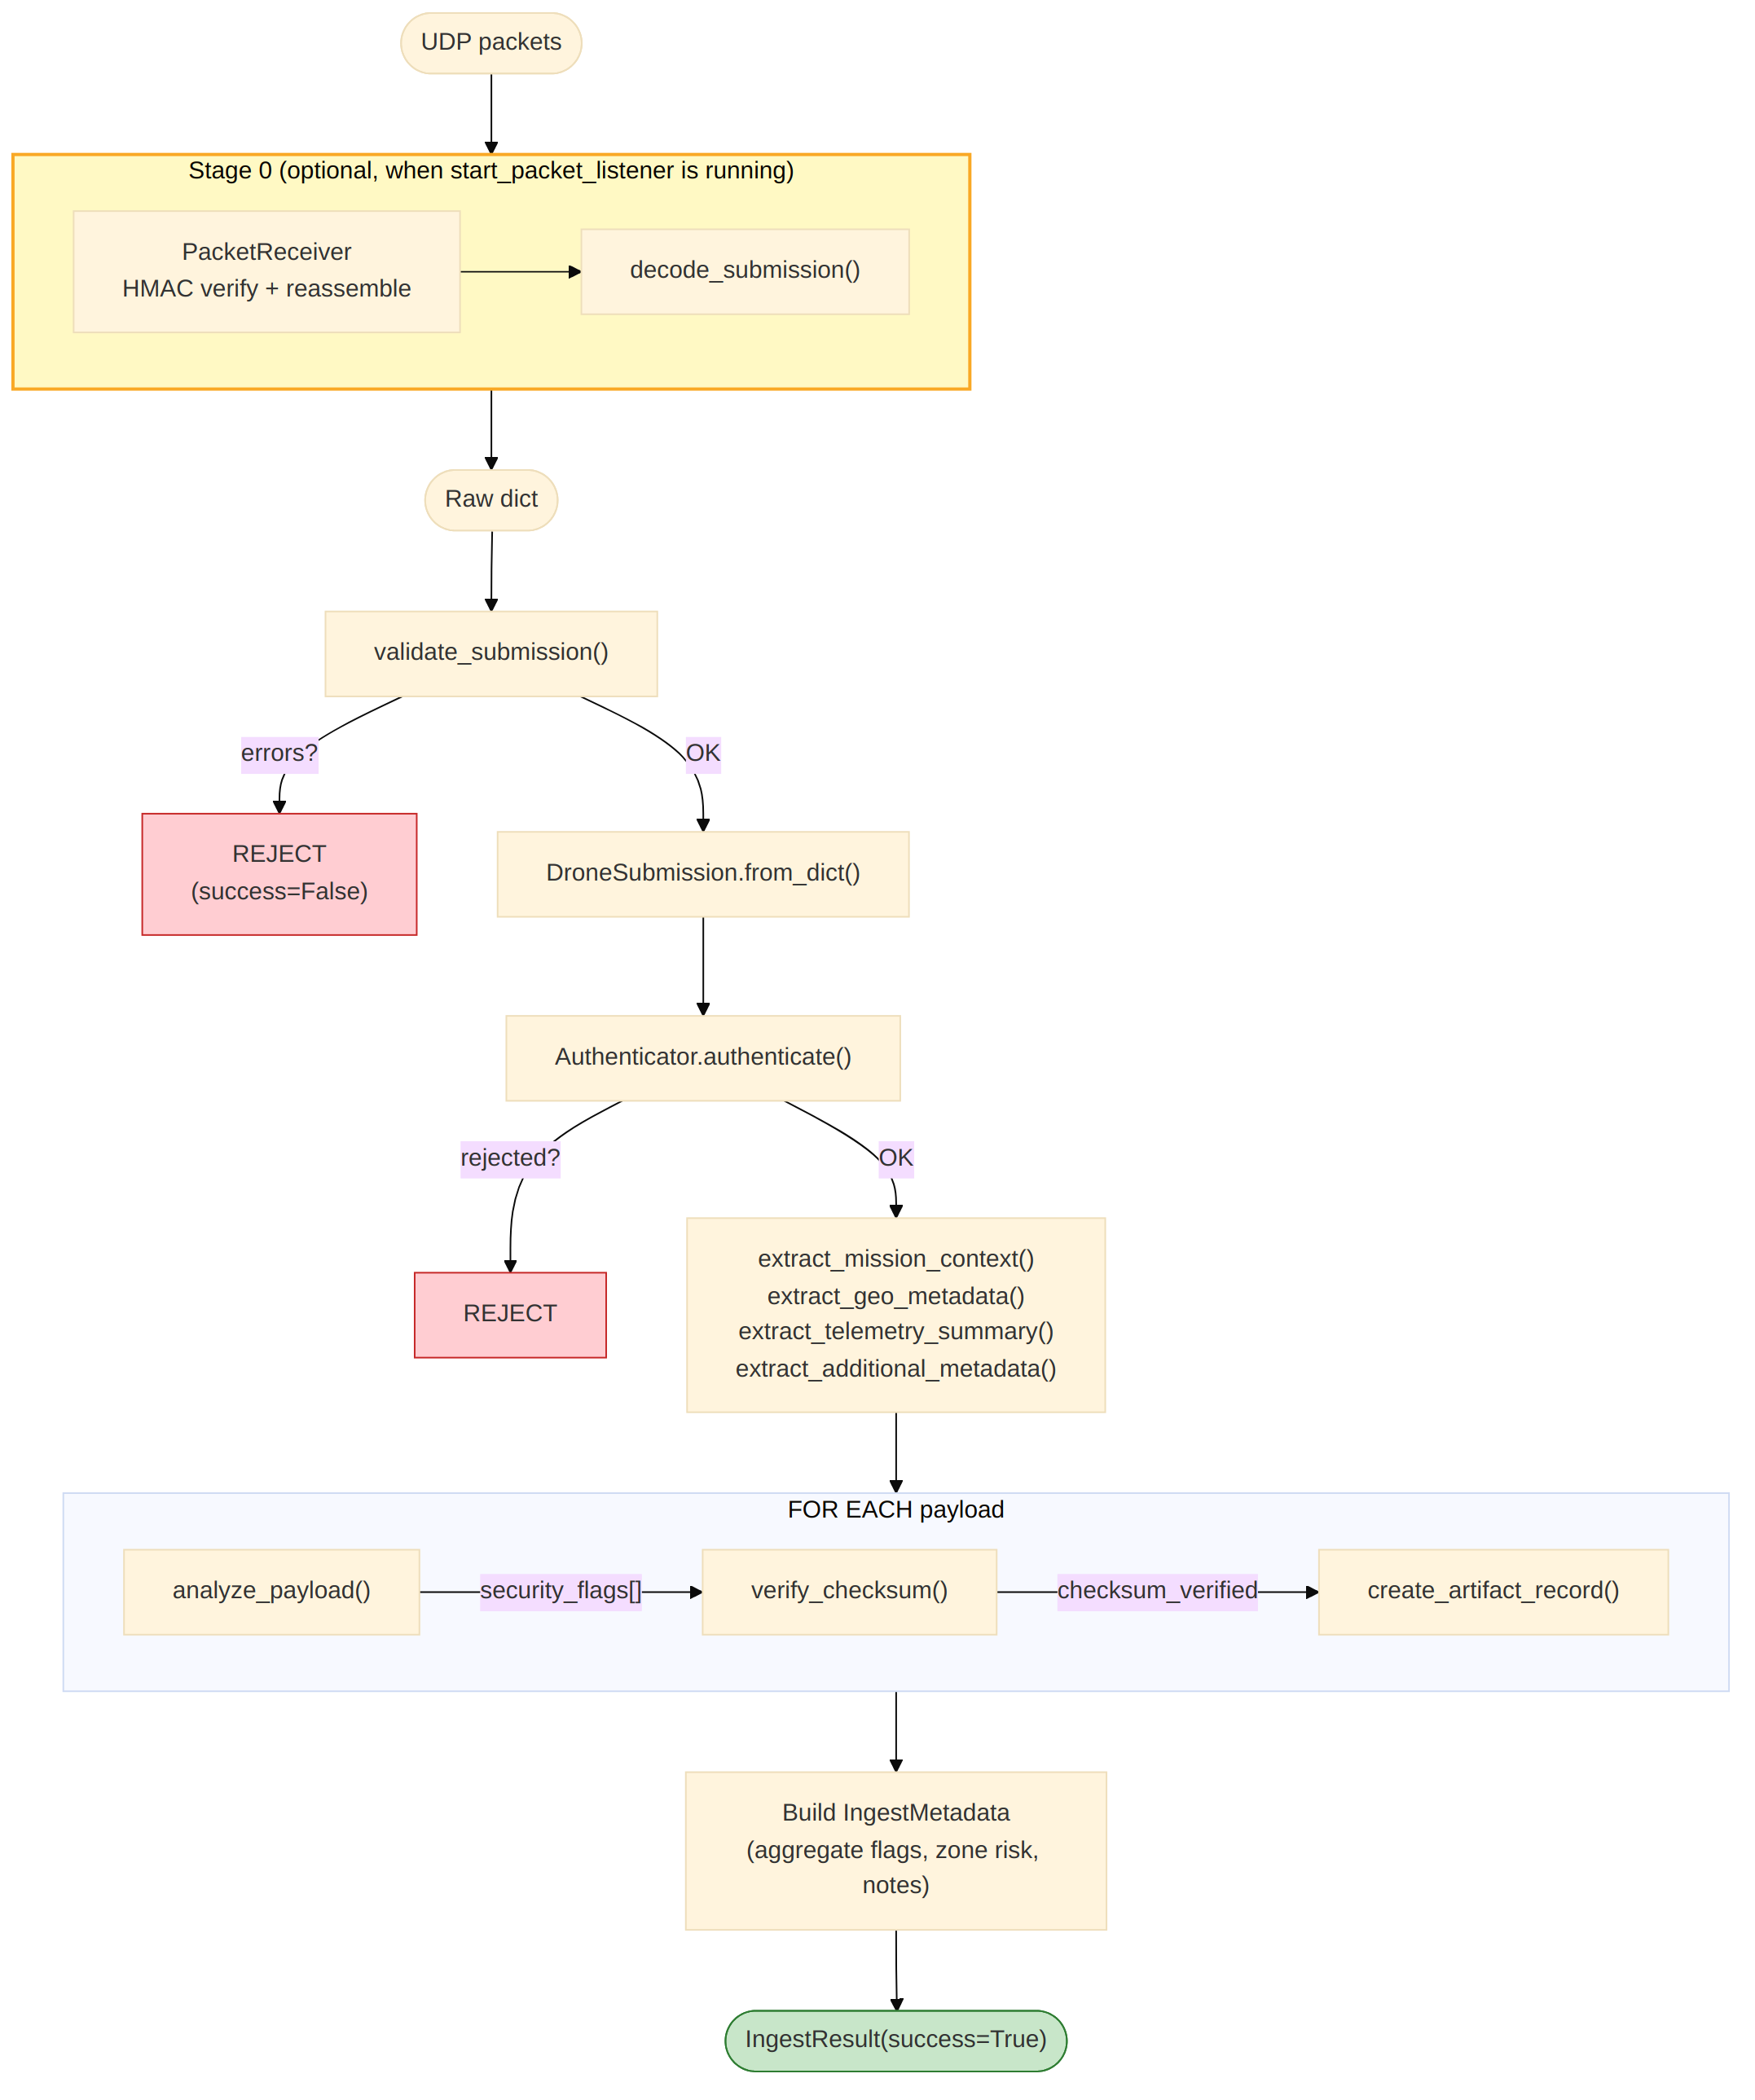
\includegraphics[width=0.85\textwidth]{ii_pipeline.png}
    \caption{Ingestion Interceptor's eight-stage pipeline.}
    \label{fig:ii_pipeline}
\end{figure}

\begin{enumerate}
    \item \textbf{Stage 0: Packet reception (optional).}
          Receives UDP packets, verifies per-packet HMAC, reassembles
          fragments, and decodes the TLV payload.
    \item \textbf{Stage 1: Validation.}
          Checks required fields (drone ID, timestamp, payloads) and ISO-8601 format.
    \item \textbf{Stage 2: Authentication.}
          Looks up the drone in a device registry and verifies its cryptographic signature (HMAC-SHA256).
    \item \textbf{Stage 3: Metadata extraction.}
          Extracts mission context, geolocation, telemetry, and additional metadata.
    \item \textbf{Stage 4: Payload analysis.}
          Flags encrypted payloads, nested archives, large binaries, suspicious MIME types, and executable extensions.
    \item \textbf{Stage 5: Checksum verification.}
          Computes and compares checksums when the source file is accessible.
    \item \textbf{Stage 6: Artifact registration.}
          Assigns a unique ID and a forensic storage pointer to each payload.
    \item \textbf{Stage 7: Output assembly.}
          Combines everything into an \texttt{IngestResult} with aggregated flags and artifact records.
\end{enumerate}

The module also supports an \textbf{uplink channel} for operator commands
(quarantine, release, revoke device, update zone risk, force rescan).

\section{Output}

Table~\ref{tab:ingest_result_fields} shows what the Interceptor produces.

\begin{table}[H]
\centering
\caption{Fields of \texttt{IngestResult}}
\label{tab:ingest_result_fields}
\begin{tabular}{|l|l|p{7cm}|}
\hline
\textbf{Field} & \textbf{Type} & \textbf{Content} \\
\hline
\texttt{ingest\_metadata} & dict & Ingest ID, drone ID, timestamp, zone, insecure flags, auth result, reputation, zone risk. \\
\hline
\texttt{artifact\_records} & list & One record per file: artifact ID, type, MIME, size, encryption flag, checksum status, storage pointer. \\
\hline
\texttt{warnings} & list & Non-fatal issues found during processing. \\
\hline
\end{tabular}
\end{table}

If validation or authentication fails, the output is an error form with a list of error strings instead.
The Threat Estimator checks for this and skips errored submissions.

\cleardoublepage

% ============================================================
% === CHAPTER 6: SANDBOX ANALYZER ===
% ============================================================

\chapter{Sandbox Analyzer}
\label{chap:sandbox}

The \textbf{Sandbox Analyzer} is Layer~3 of the detection engine. It runs only
when the Threat Estimator scores a submission as High. It executes the
suspicious file inside a kernel-limited Linux sandbox, watches it through four
\texttt{/proc}-based monitors, scores the observed behaviour, and returns a
verdict: \emph{Clean}, \emph{Suspicious}, or \emph{Malicious}.

\section{Design Principles}

\begin{enumerate}
    \item \textbf{Magic-byte routing.} Extensions are never trusted. The first
          16 bytes decide the true file type; a \texttt{photo.jpg} starting
          with \texttt{\#!} is treated as a script.
    \item \textbf{Encrypted archives are evidence.} No dictionary attacks.
          An encrypted ZIP without a declared key adds risk points and skips
          extraction.
    \item \textbf{Kernel-level isolation.} Resource caps
          (\texttt{RLIMIT\_AS}, \texttt{RLIMIT\_CPU}, \texttt{RLIMIT\_FSIZE},
          \texttt{RLIMIT\_NPROC}, \texttt{RLIMIT\_CORE}) are set via
          \texttt{preexec\_fn} before the target runs. Monitoring reads
          \texttt{/proc} from outside, so the process cannot fake it.
\end{enumerate}

\section{Eight-Stage Pipeline}

Figure~\ref{fig:sb_pipeline} shows the flow.
Table~\ref{tab:sb_stages} lists each stage.

\begin{figure}[H]
    \centering
    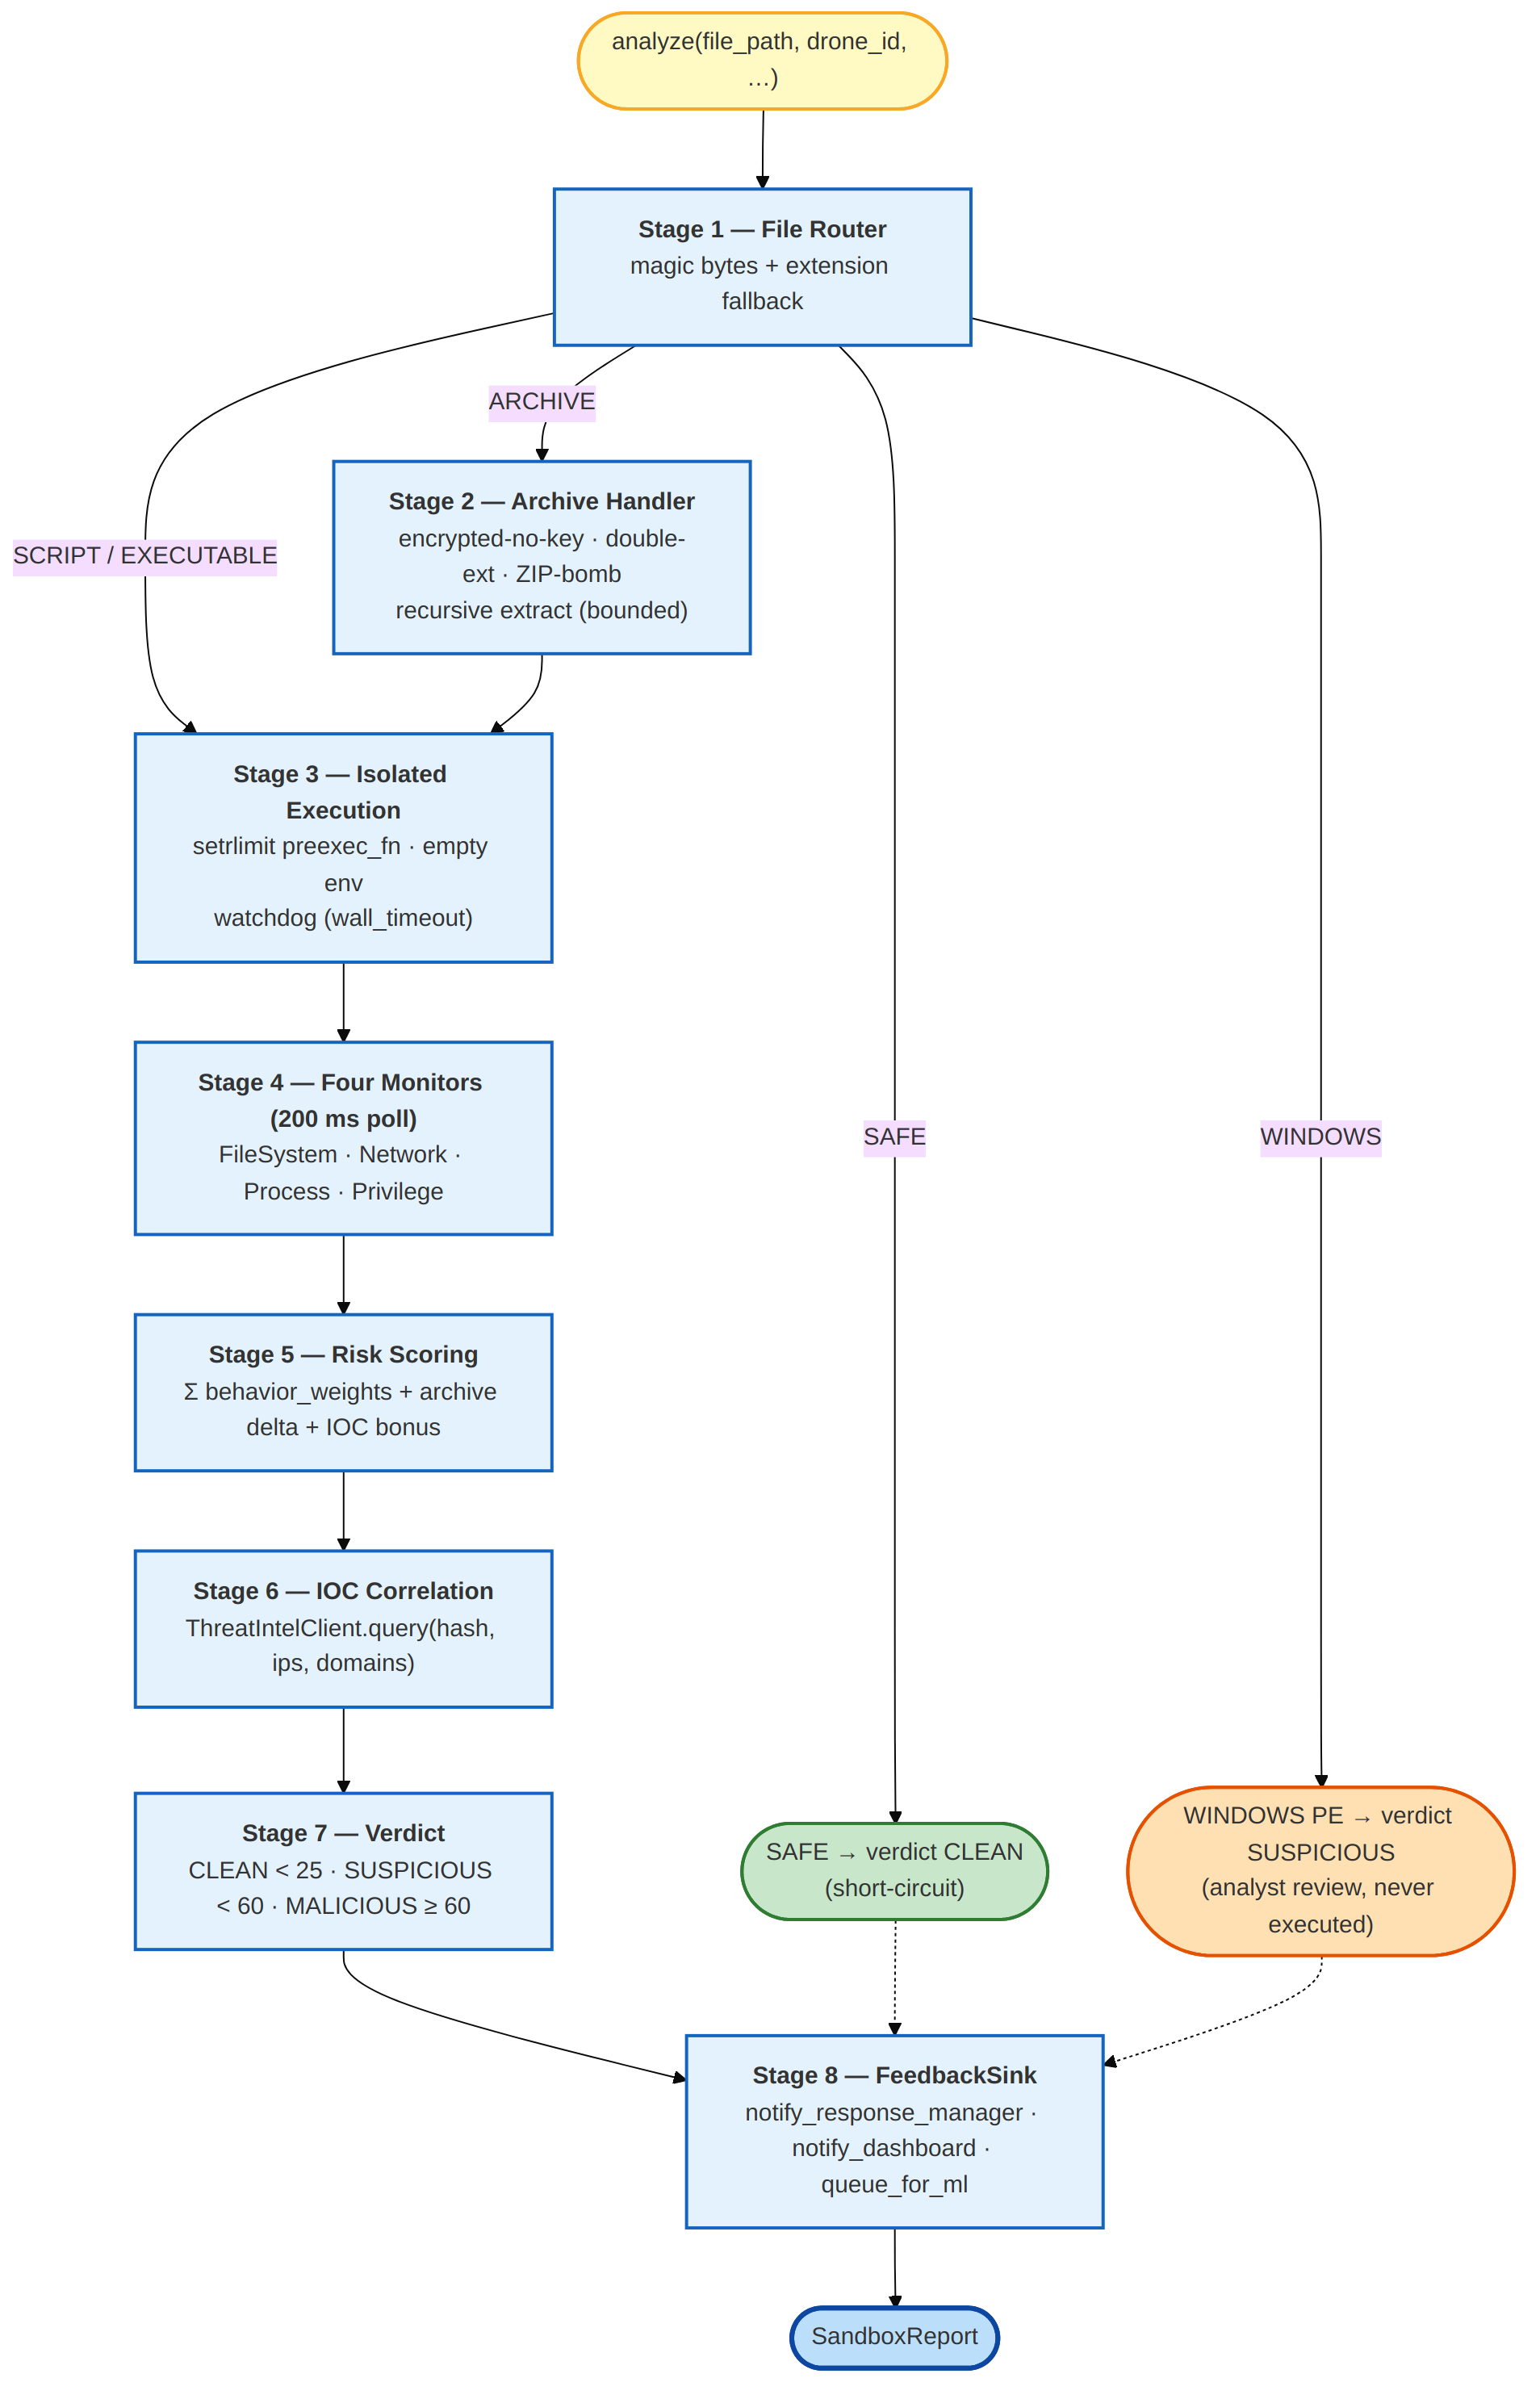
\includegraphics[width=0.78\textwidth]{sb_pipeline.png}
    \caption{Sandbox Analyzer pipeline with short-circuits for safe and Windows files.}
    \label{fig:sb_pipeline}
\end{figure}

\begin{table}[H]
\centering
\caption{Sandbox pipeline stages}
\label{tab:sb_stages}
\begin{tabular}{|c|l|p{8.2cm}|}
\hline
\textbf{\#} & \textbf{Stage} & \textbf{Purpose} \\
\hline
1 & File Router & Magic bytes with extension fallback. SAFE files $\to$ Clean, Windows PE $\to$ Suspicious. \\
\hline
2 & Archive Handler & Encrypted-no-key (+25 risk), double-extension (+30), ZIP bomb detection. Recurse up to depth 3. \\
\hline
3 & Isolated Execution & \texttt{setrlimit} caps (128 MB RAM, 20 s CPU, 32 MB file, 50 procs), empty env, 30 s watchdog. \\
\hline
4 & Four Monitors & File System, Network, Process, and Privilege monitors poll \texttt{/proc} every 200 ms. \\
\hline
5 & Risk Scoring & Sum of per-event weights + archive bonus + IOC bonus. \\
\hline
6 & IOC Correlation & SHA-256, observed IPs, and domains checked against a \texttt{ThreatIntelClient}. \\
\hline
7 & Verdict & $< 25$ Clean, $25$--$59$ Suspicious (quarantine), $\geq 60$ Malicious (block). \\
\hline
8 & Feedback & Sends report to Response Manager, Dashboard, and ML retraining queue. \\
\hline
\end{tabular}
\end{table}

\section{Monitoring}

Four monitors run in parallel while the file executes.
Table~\ref{tab:sb_monitors} shows what each one watches.

\begin{table}[H]
\centering
\caption{The four monitors}
\label{tab:sb_monitors}
\begin{tabular}{|l|p{4.3cm}|p{5.5cm}|}
\hline
\textbf{Monitor} & \textbf{Source} & \textbf{Events raised} \\
\hline
File System & \texttt{/proc/<PID>/fd} + \texttt{fdinfo} & \texttt{file\_system\_write}, \texttt{file\_write\_executable} \\
\hline
Network & \texttt{/proc/net/tcp} baseline diff & \texttt{network\_connect} (catches C2 callbacks even if they fail) \\
\hline
Process & \texttt{psutil} child-tree walk & \texttt{process\_spawn}, \texttt{shell\_command} \\
\hline
Privilege & \texttt{/proc/<PID>/status} & \texttt{privilege\_escalation}, \texttt{memory\_inject} \\
\hline
\end{tabular}
\end{table}

\section{Risk Scoring and Verdict}

Each event adds its weight to the total score. Table~\ref{tab:sb_weights}
lists the weights. The approach follows Cuckoo Sandbox's additive
pattern~\cite{bayer2009scalable}.

\begin{table}[H]
\centering
\caption{Default behaviour weights}
\label{tab:sb_weights}
\begin{tabular}{|l|c||l|c|}
\hline
\textbf{Category} & \textbf{Wt} & \textbf{Category} & \textbf{Wt} \\
\hline
\texttt{self\_replication} & 40 & \texttt{shell\_command} & 25 \\
\hline
\texttt{privilege\_escalation} & 35 & \texttt{high\_entropy\_write} & 15 \\
\hline
\texttt{memory\_inject} & 35 & \texttt{dns\_lookup} & 15 \\
\hline
\texttt{file\_write\_executable} & 30 & \texttt{process\_spawn} & 10 \\
\hline
\texttt{api\_hooking} & 30 & \texttt{file\_delete} & 10 \\
\hline
\texttt{network\_connect} & 25 & \texttt{file\_system\_write} & 5 \\
\hline
\end{tabular}
\end{table}

Verdict bands: \textbf{Clean} ($< 25$), \textbf{Suspicious} ($25$--$59$,
quarantine for analyst review), \textbf{Malicious} ($\geq 60$, block and
alert SOC)

\cleardoublepage

% ============================================================
% === CHAPTER 7: METADATA SANITIZER ===
% ============================================================

\chapter{Metadata Sanitizer}
\label{chap:metadata_sanitizer}

The \textbf{Metadata Sanitizer} cleans embedded metadata from drone
payload files. It strips harmful fields from EXIF data in images,
JavaScript in PDFs, tracking atoms in videos, and hidden entries in
archives. The original file is always preserved as a forensic copy,
and every change is recorded with before-and-after SHA-256 hashes.
After cleaning, the file is re-parsed to confirm it is still valid.

\section{Sanitization Modes}

The sanitizer supports three modes. The mode is picked automatically
from the Threat Score ($T_S$) received from the Game-Theoretic Threat
Estimator:

\begin{itemize}
    \item $T_S \geq 0.7$ $\to$ \textbf{Strip:} remove all non-essential metadata.
    \item $T_S \leq 0.3$ $\to$ \textbf{Audit-only:} log dangerous fields without modifying the file.
    \item Otherwise $\to$ \textbf{Selective} (default): remove only known-dangerous fields.
\end{itemize}

If the Ingestion Interceptor's insecure flags include high-risk markers
(e.g.\ \emph{encrypted\_payload}), the mode is escalated to Strip
regardless of the Threat Score. An explicit mode override from the
caller always takes priority.

\section{File-Type Handlers}

Each file type has a dedicated handler. Table~\ref{tab:handlers} lists
the built-in handlers and what they clean.

\begin{table}[H]
\centering
\caption{Built-in file-type handlers and their cleanup actions}
\label{tab:handlers}
\begin{tabular}{|l|l|p{7cm}|}
\hline
\textbf{Handler} & \textbf{Types} & \textbf{What it strips} \\
\hline
Image & JPEG, PNG, TIFF, BMP & EXIF / XMP / IPTC blocks (GPS, UserComment, MakerNote, CameraSerialNumber). \\
\hline
PDF & PDF & JavaScript, auto-open actions (/OpenAction, /AA), embedded files, /Launch. \\
\hline
Video & MP4, MKV, MOV, MP3, FLAC & Tracking atoms (meta, loci), device identifiers, vendor-specific boxes. \\
\hline
Archive & ZIP, TAR & Hidden members, comments, dirty central directory entries. \\
\hline
Text & TXT, CSV, JSON & Unicode direction-override characters, line-ending normalisation. \\
\hline
\end{tabular}
\end{table}

Rules are organised into three declarative lists per file type:
\emph{always strip}, \emph{strip in high-security mode}, and
\emph{always preserve}. Operators can extend these lists without
modifying code.

\section{Output}

For each file the sanitizer returns a result containing: the mode used,
the list of changes (field, action, reason, severity), before/after
metadata hashes, warnings, errors, and whether the file passed
post-sanitization verification. Batch results aggregate per-file totals
(processed, sanitised, skipped, errors, total changes).

\cleardoublepage

% ============================================================
% === CHAPTER 8: RESULTS AND ANALYSIS ===
% ============================================================

\chapter{Results and Analysis}
\label{chap:results}

All experiments used synthetic drone payloads on commodity Linux
hardware with Python 3.10. Six representative samples were used:
normal video+image (A), encrypted nested ZIP (B), telemetry-only (C),
large survey video (D), double-extension archive (E), and a C2
callback script (F).

\section{Threat Estimator Results}

\textbf{Bayesian cold-start.}
The reference example (ZIP from a risky zone, $P(N) = 0.85$)
gives $R \approx 0.257$, matching the expected value.
Table~\ref{tab:gte_bayes} shows the cold-start reputations for all
samples.

\begin{table}[H]
\centering
\caption{Cold-start Bayesian reputations}
\label{tab:gte_bayes}
\begin{tabular}{@{}llll@{}}
\toprule
\textbf{Sample} & \textbf{Zone} & \textbf{File type} & \textbf{$R$} \\
\midrule
A & zone-a & video & 0.988 \\
B & zone-c & archive & 0.257 \\
C & zone-b & telemetry & 0.969 \\
D & zone-a & video & 0.988 \\
E & zone-3 & archive & 0.257 \\
\bottomrule
\end{tabular}
\end{table}

\textbf{Threat Score.}
Table~\ref{tab:gte_results} shows the end-to-end scores after the
Stackelberg solver and sigmoid blend.

\begin{table}[H]
\centering
\caption{Threat Score and inspection level}
\label{tab:gte_results}
\begin{tabular}{@{}lccl@{}}
\toprule
\textbf{Sample} & \textbf{Source} & \textbf{$T_S$} & \textbf{Level} \\
\midrule
A & bayesian\_prior & 0.011 & Low \\
B & bayesian\_prior & 0.075 & Low \\
C & bayesian\_prior & 0.624 & Medium \\
D & bayesian\_prior & 0.011 & Low \\
E & bayesian\_prior & 0.075 & Low \\
\bottomrule
\end{tabular}
\end{table}

\textbf{Adaptive thresholds.}
Under a synthetic feedback sequence where FPR dropped from $0.12$ to
$0.05$, the thresholds drifted from $(0.40, 0.70)$ to $(0.415, 0.715)$
without leaving the safe bounds. Elevated FNR moved them in the
opposite direction.

\textbf{Reputation dynamics.}
Starting from $R_0 = 0.257$, one malicious verdict drove $R$ down to
$0.128$. Ten benign verdicts recovered it to $0.555$, confirming
the asymmetric design ($\eta_+ = 0.05$, $\eta_- = 0.50$).

\section{Ingestion Interceptor Results}

All six samples were processed without error (75 tests pass).
Table~\ref{tab:ii_flags} shows the extracted insecure flags.

\begin{table}[H]
\centering
\caption{Insecure flags extracted by the Ingestion Interceptor}
\label{tab:ii_flags}
\begin{tabular}{@{}lcl@{}}
\toprule
\textbf{Sample} & \textbf{Count} & \textbf{Flags} \\
\midrule
A & 0 & (none) \\
B & 2 & encrypted\_payload, nested\_archive \\
C & 0 & (none) \\
D & 1 & large\_binary \\
E & 1 & suspicious\_mime \\
F & 0 & (none) \\
\bottomrule
\end{tabular}
\end{table}

The Stage~0 packet receiver was tested separately with a drone
simulator. Fragmented, HMAC-signed UDP streams were reassembled
correctly; malformed and replayed packets were dropped as expected.

\section{Sandbox Analyzer Results}

Table~\ref{tab:sb_demo} shows the sandbox outcomes (50 tests pass).

\begin{table}[H]
\centering
\caption{Sandbox Analyzer demo outcomes}
\label{tab:sb_demo}
\begin{tabular}{|p{4cm}|l|c|c|p{4.5cm}|}
\hline
\textbf{Scenario} & \textbf{Category} & \textbf{Score} & \textbf{Verdict} & \textbf{Notes} \\
\hline
Safe CSV & safe & 0 & Clean & Short-circuited at Stage 1. \\
\hline
Disguised \texttt{.jpg} script & script & 0 & Clean & Caught by magic bytes. \\
\hline
Archive with \texttt{recon.jpg.sh} & archive & 85 & Malicious & Double-ext + network event. \\
\hline
Python C2 callback & script & 75 & Malicious & \texttt{network\_connect} $\times 3$. \\
\hline
Windows PE & windows & 0 & Suspicious & Not executed; quarantined. \\
\hline
\end{tabular}
\end{table}

Windows PE files are short-circuited to Suspicious because inability
to analyse is not evidence of safety.

\section{Metadata Sanitizer Results}

Table~\ref{tab:ms_results} shows sample results (96 tests pass).

\begin{table}[H]
\centering
\caption{Metadata Sanitizer results}
\label{tab:ms_results}
\begin{tabular}{|p{4cm}|l|p{3.5cm}|c|}
\hline
\textbf{Input} & \textbf{Mode} & \textbf{Changes} & \textbf{Valid?} \\
\hline
JPEG (GPS + UserComment) & selective & 2 (GPS, UserComment) & yes \\
\hline
PDF (JS + OpenAction) & selective & 2 (JS, OpenAction) & yes \\
\hline
MP4 (loci + vendor atom) & selective & 1 (loci) & yes \\
\hline
ZIP (clean) & audit\_only & 0 & yes \\
\hline
EXE (skipped MIME) & skip & 0 & n/a \\
\hline
\end{tabular}
\end{table}

Mode selection was verified: $T_S < 0.3$ picked audit-only, $T_S > 0.7$
picked strip, and intermediate scores picked selective. Explicit mode
overrides took priority.

\cleardoublepage

% ============================================================
% === CHAPTER 9: CONCLUSION AND FUTURE WORK ===
% ============================================================

\chapter{Conclusion and Future Work}
\label{chap:conclusion}

\section{Summary}

This project built four modules of a multi-layered threat detection
pipeline for drone data streams:

\begin{enumerate}
    \item \textbf{Game-Theoretic Threat Estimator:} Stackelberg game
          + Bayesian cold-start reputation + adaptive thresholds.
    \item \textbf{Ingestion Interceptor:} 8-stage pipeline with
          authentication, metadata extraction, flag detection, and
          UDP packet reception.
    \item \textbf{Sandbox Analyzer:} kernel-limited execution with
          four \texttt{/proc} monitors, risk scoring, and three-level
          verdict.
    \item \textbf{Metadata Sanitizer:} strips dangerous metadata
          from images, PDFs, videos, and archives with mode driven by
          the Threat Score.
\end{enumerate}

\section{Limitations}

\begin{itemize}
    \item The remaining five pipeline modules (Signature Scanner, AI/ML
          Classifier, Threat Intelligence Correlator, Response Manager,
          Dashboard) are outside the scope of this work; the four
          modules expose integration seams for them.
    \item The sandbox needs Linux (\texttt{setrlimit} + \texttt{/proc});
          Windows PE files are flagged but not executed.
    \item Bayesian CPTs are seed values from operational intuition, not
          learned from a labelled dataset.
    \item All evaluations use synthetic payloads, not live drone feeds.
\end{itemize}

\section{Future Work}

\begin{itemize}
    \item \textbf{Complete system integration:} wire the four modules
          with the remaining five (Signature Scanner, AI/ML Classifier,
          Threat Intelligence Correlator, Response Manager, Dashboard)
          into a single deployable pipeline.
    \item \textbf{Testing with real drones:} replace the drone
          simulator with actual drone feeds (MAVLink, DJI MSDK) and
          validate on real mission data.
    \item \textbf{Deployment on edge hardware:} deploy the full
          pipeline on field edge nodes and measure long-run accuracy,
          latency, and stability.
    \item \textbf{Feedback loop with real verdicts:} learn the
          Bayesian CPTs and retune scoring weights from analyst-confirmed
          detection outcomes instead of synthetic feedback.
    \item \textbf{Production persistence:} replace the in-memory
          reputation store with a database-backed store for restart
          resilience.
    \item \textbf{Windows sandbox:} add a VM-based backend so
          Windows PE files can be executed and analysed.
\end{itemize}

\cleardoublepage

% ============================================================
% === REFERENCES ===
% ============================================================

\addcontentsline{toc}{chapter}{References}
\bibliographystyle{ieeetr}

\nocite{*}

\bibliography{references}

\end{document}
